\chapter{Estado del arte}
\label{chap:estado_arte}

\drop{E}{  n} este capítulo se presentarán y describirán las principales áreas en las que este \acs{TFM} se ha basado; \textbf{Historia del Arte}, \textbf{Realidad Virtual}, \textbf{Diseño 3D} y \textbf{Desarrollo de Videojuegos}.

Uno de los retos que ha supuesto este proyecto ha sido el de estudiar y comparar las diferentes alternativas que se presentaban a la hora de resolver un determinado problema; por ello, en los casos en los que esto aplique se presentarán las diferentes opciones disponibles que han sido estudiadas.

La descripción de estado del arte de cada una de las áreas en las que se ha basado este trabajo comenzará con un recorrido general a lo largo de su historia, hablando de sus contribuciones y posibilidades para terminar presentando su estado actual. Por ello, el estudio de cada una de las áreas mencionadas se dividirá y se detallará a través de sus subáreas, lo que permitirá un estudio más profundo y más detallado de la misma.

La sección de la \textbf{Historia del Arte} comenzará exponiendo un breve recorrido por sus diferentes etapas de manera crónica. Además, se explicará el origen del nombre de este \acs{TFM}.

A continuación, en la sección de la \textbf{Realidad Virtual} se hablará de su historia, las tecnologías y recursos software disponibles y de las interfaces con las que pueden interactuar los usuarios de esta tecnología.

La siguiente sección hablará del \textbf{Diseño 3D}, de qué programas y suites existen actualmente para modelar tridimensionalmente y qué \acs{IDE}s hay disponibles para desarrollar e implementar sistemas interactivos.

Por último, se hablará del \textbf{Desarrollo de Videojuegos} y de sus aplicaciones en este proyecto desde un punto de vista teórico.

La figura \ref{fig:mapa-conceptual} ofrece un resumen de las diferentes tecnologías que colaboran en \MineRVa y de las relaciones que hay entre ellas.

\vspace{0.4cm}

\begin{figure}[!h]
    \begin{center}
        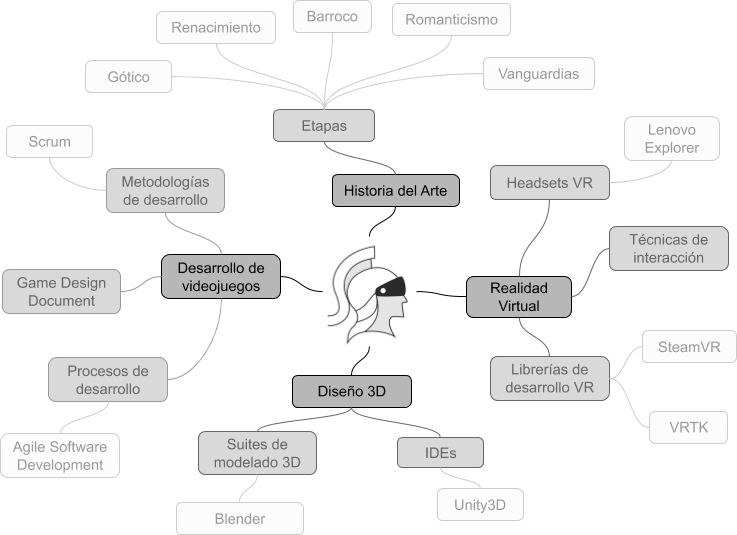
\includegraphics[width=1\textwidth]{imagenes/2/mapa-conceptual.png}
        \caption{Mapa conceptual de \MineRVa}
        \label{fig:mapa-conceptual}
    \end{center}
\end{figure}

\section{Historia del Arte}

Para entender el contexto artístico de este \acs{TFM} primero se presentará un breve resumen a través de las etapas del Arte \cite{ramirez-0610}.

\subsection{Prehistórico}

Habría que remontarse a la etapa prehistórica más antigua, el \textbf{Paleolítico}, para encontrar las primeras muestras de arte. Los primeros homínidos plasmaron su realidad en las paredes de las cuevas y abrigos que habitaron, legándonos lo que hoy conocemos con el nombre de \textbf{pinturas rupestres}. Sirviéndose de pigmentos naturales, grasa animal, carbón y sangre, representaron grupos humanos danzantes y escenas de cacerías con un sentido mágico y sagrado, al existir la creencia de que favorecían la fertilidad de las mujeres de la tribu o fomentaban la caza. El mismo cometido tenían las toscas estatuillas realizadas en piedra y hueso, que con el tiempo fueron sustituidas por otras más refinadas. Por tanto, lo que hoy catalogamos como producciones artísticas a las que atribuimos un valor estético, no fueron ideadas como tal, sino que cumplían una función concreta como medio para obtener ganancias materiales.

\subsection{Mesopotámico y precolombino}

Será en la antigua región de \textbf{Mesopotamia} donde encontremos el origen de la civilización en los términos en los que hoy la entendemos y un arte más acorde con la concepción actual. Las numerosas culturas que se sucedieron en este reducido punto geográfico levantaron una arquitectura pensada y medida, digna de grandes ingenieros capaces de proyectar edificios de gran envergadura, sus conocidos \textit{zigurats}, figura \ref{fig:zigurat} (antecedentes de las pirámides egipcias), por medio de sistemas de arcos y bóvedas. Las artes plásticas no se quedaron atrás. Hoy en día se conservan restos escultóricos y relieves de gran calidad técnica, que han marcado una etapa tan florida como misteriosa de nuestra historia.

\begin{figure}[!h]
    \begin{center}
    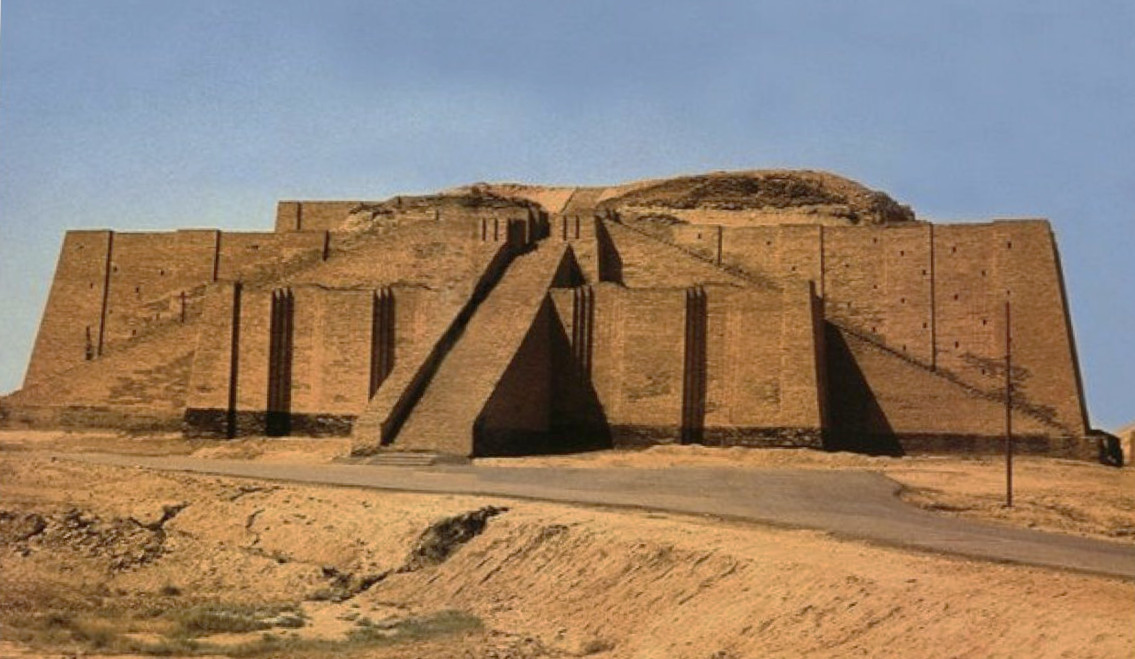
\includegraphics[width=0.7\textwidth]{imagenes/2/zigurat.jpg}
    \caption{\textit{Zigurat} de \textit{Uruk}, 3200-3000 a. C.}
    \label{fig:zigurat}
    \end{center}
\vspace{-0.4cm}
\end{figure}

Paralelamente, cabe destacar la importancia de las manifestaciones artísticas que están teniendo lugar en el continente americano. Los templos \textbf{incas y mayas} son solo un ejemplo del ingenio y la habilidad de aquellas civilizaciones.

\subsection{Arte clásico}

Los \textbf{griegos} abrieron paso a un nuevo tipo de arte basado en la medida humana: la arquitectura está hecha por y para el hombre, y tanto la escultura como la pintura están protagonizadas por la figura humana, en la que reinan los ideales de armonía y proporción. 

Los \textbf{romanos}, muy influenciados por los anteriores, erigieron una arquitectura grandilocuente a la vez que funcional, pensada para el disfrute de los grandes hombres de la época y la exaltación de su poder, igual que los arcos de triunfo y los monumentos conmemorativos. La escultura, heredera de la griega, se vuelve más realista y poderosa.

El nombre de este \acs{TFM} viene de la \textbf{deidad romana Minerva}, que es la \textbf{diosa del arte}, la sabiduría y la guerra, además de la protectora de Roma y la patrona de los artesanos. El poeta Ovidio se refería a Minerva como \textit{la diosa de las mil obras} \cite{lomb-13}. Su equivalente en la mitología griega es Atenea.

\subsection{Arte medieval}

El \textbf{arte islámico} se extendió por Próximo Oriente y avanzó hasta la Península Ibérica, donde los musulmanes permanecieron durante ocho siglos (711-1492). En función de sus zonas de dominio emprendieron un arte muy dispar, centrando sus esfuerzos en la arquitectura especialmente. Fue característico de sus construcciones el uso del arco apuntado, el lobulado y sus variantes, y el arco de herradura, este último sobre todo en la Península dada la influencia visigoda en nuestro territorio. Las yeserías de entramados vegetales, las tracerías, la eboraria y la incorporación del agua y de la naturaleza en la obra artística son otros rasgos distintivos del arte islámico. Ejemplo de ello es el Alcázar de Sevilla, que puede verse en la figura \ref{fig:patio-doncellas}.

\begin{figure}[!h]
    \begin{center}
        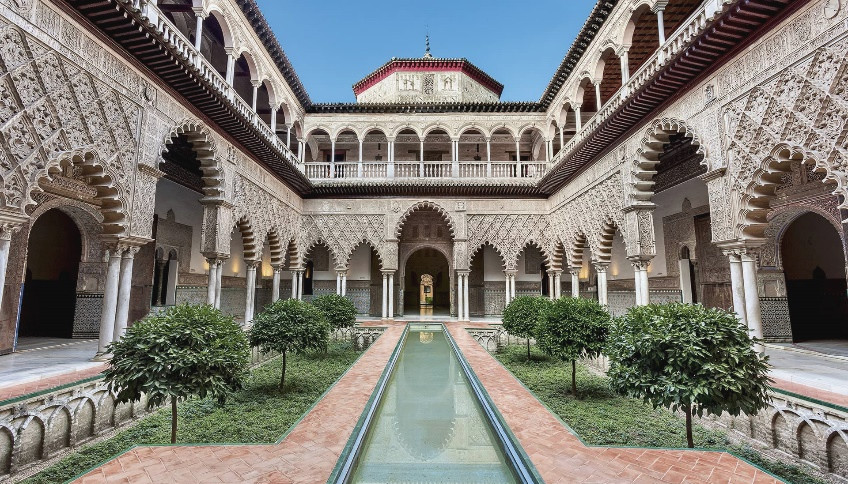
\includegraphics[width=0.7\textwidth]{imagenes/2/patio-doncellas.jpg}
        \caption{Patio de las Doncellas del Alcázar de Sevilla, siglo X}
        \label{fig:patio-doncellas}
    \end{center}
\end{figure}

La llegada de la \textbf{Edad Media} en Europa después de la caída del Imperio Romano de Occidente y la irrupción del cristianismo como nueva religión dominante tuvieron una repercusión directa en el arte generado a partir del siglo V en Europa. La cristiandad encontrará en el \textbf{arte paleocristiano} su primera manifestación, en un principio clandestina, a través de los sarcófagos y pinturas de catacumbas y, tras la legalización de la religión, de manera pública a través de las grandes basílicas. 

Pero fue en el \textbf{románico}, primer estilo internacional de la cultura occidental, donde el cristianismo se manifestó de manera total a partir del siglo X. La arquitectura se caracterizó, en general, por la sencillez estructural, basándose en gran medida en la producida por los romanos. La profusión decorativa se concentró en espacios muy concretos de los edificios, como las grandes portadas de las iglesias, adornadas con conjuntos escultóricos centrados en la vida de Jesús, la Virgen María y los Santos patrones, algunos de gran complejidad iconográfica. La escultura, al igual que la pintura, se caracterizó por la sencillez de las formas y el hieratismo de gestos y actitudes: el naturalismo no era una prioridad para los promotores de las obras, más interesados en la expresión espiritual de las figuras.

Las formas simples del románico se fueron complicando progresivamente hasta culminar en un nuevo estilo, el \textbf{gótico}, caracterizado por la verticalidad, la luminosidad y la mayor riqueza ornamental. Los avances constructivos posibilitaron la edificación de templos de mayor altura y vanos cada vez más amplios que se cubrieron con vidrieras. En cuanto a las artes plásticas, prevalece la costumbre de colmatar las portadas de acceso con importantes ciclos iconográficos esculpidos. La escultura se volvió más naturalista en estas fechas, rompiendo con la rigidez románica aunque manteniendo el halo de espiritualidad. La pintura recubrió los muros de las iglesias y se traspasó también a la tabla y a la miniatura, que iluminó los libros litúrgicos.

\subsection{Renacentismo}

Con el Renacimiento se volvió la mirada a la época clásica, recuperando el arte a la medida del hombre. Los artistas comenzaron a ser reconocidos como trabajadores intelectuales y dejaron de ser considerados como simples artesanos. Fue el momento de grandes arquitectos como Brunelleschi y Alberti, que erigieron grandes templos cristianos inspirándose en las magníficas obras romanas; escultores de la talla de Donatello, que ejecutó obras realistas con buenas dosis de idealización a la manera clásica; y pintores como Botticelli y Piero della Francesca, introductor de la perspectiva. Otros artistas pasaron a la historia como grandes hombres del Renacimiento polifacéticos e inclasificables: Leonardo da Vinci, Rafael o Miguel Ángel Buonarroti, cuya obra más famosa es la Capilla Sixtina (figura \ref{fig:capilla-sixtina}). 

\begin{figure}[!h]
    \begin{center}
        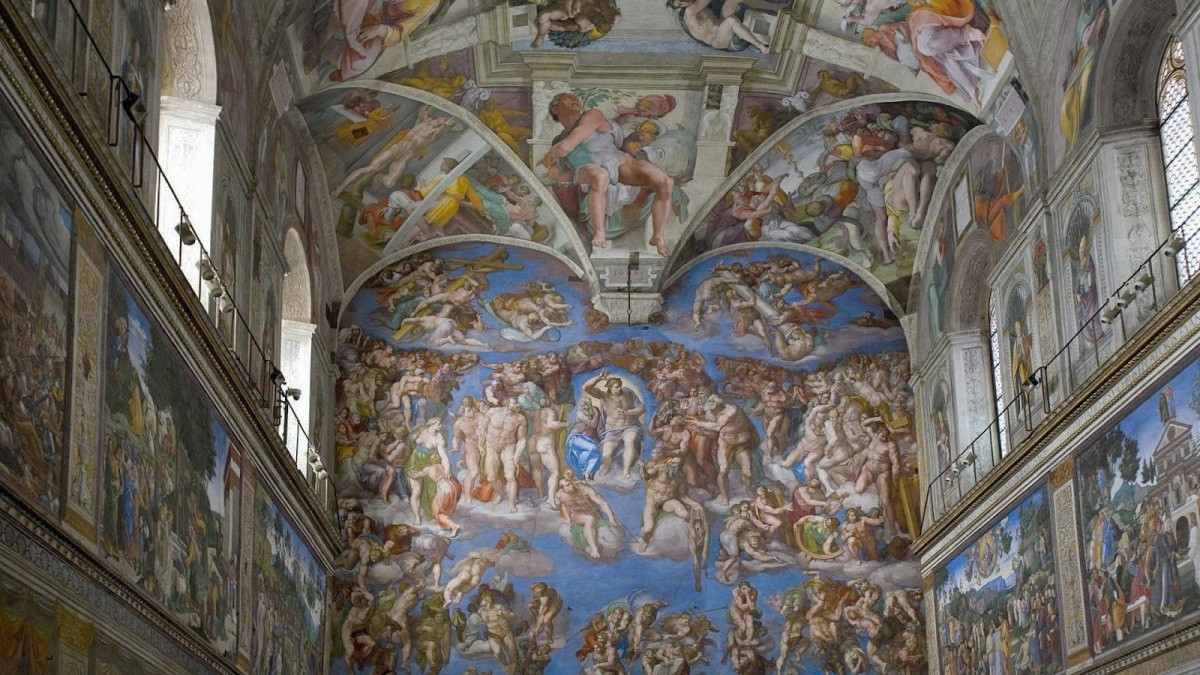
\includegraphics[width=0.7\textwidth]{imagenes/2/capilla-sixtina.jpg}
        \caption{Miguel Ángel Buonarroti, \textit{Capilla Sixtina}, 1508-1512}
        \label{fig:capilla-sixtina}
    \end{center}
\end{figure}

\subsection{Barroco}

La última etapa renacentista del Manierismo fue revelando lo que ocurriría con las artes a partir del siglo XVII. El Barroco fue la etapa de eclosión de una arquitectura grandilocuente y teatral que cumplió con una doble función: por un lado, la de manifestar el poder de los comitentes de la obra, que utilizaban la arquitectura como auténtica propaganda política; y por otro lado, en la arquitectura religiosa, la de adoctrinar a unos fieles fácilmente impresionables. Las iglesias se recubrieron de pinturas murales, que ocuparon también las bóvedas a modo de rompimientos celestes, y de ciclos escultóricos que representaron la vida de Cristo y de los Santos, sirviendo sus figuras como modelos de vida. La pintura encontró en esta época su momento más destacado hasta la fecha en cuanto a técnica y revaloración social. Pintores de la talla de Caravaggio en Italia o de Velázquez en España introdujeron una nueva manera de plasmar el mundo a través de unas composiciones cada vez más complejas y la técnica del claroscuro.

\subsection{Siglo XIX}

En sus últimos momentos, el Barroco adquiere una profusión decorativa y un nivel de recargamiento inusitados en la Historia de los estilos. Los arquitectos del siglo XIX vinieron a romper con esta grandilocuencia y condujeron a la arquitectura hacia el academicismo y la mesura. No obstante, no se puede hablar de homogeneidad estilística en toda la centuria. La arquitectura, si se caracterizó por algo, fue por el eclecticismo y la recuperación de tendencias pasadas a través de los historicismos. Así, volvemos a encontrar cresterías en el Neogótico, grandes órdenes arquitectónicos en el Neoclásico o rasgos de inspiración hispanomusulmana en el Neomudéjar, entre otros.

Lo mismo ocurrió con la pintura. La mayor libertad en el sistema artístico permitió que los artistas elaboraran unos estilos cada vez más personales, dando lugar a unas producciones muy dispares. Románticos, realistas, impresionistas, simbolistas, y un largo etcétera hicieron de este siglo uno de los más prolíficos y originales hasta el momento.

\begin{figure}[!h]
    \begin{center}
        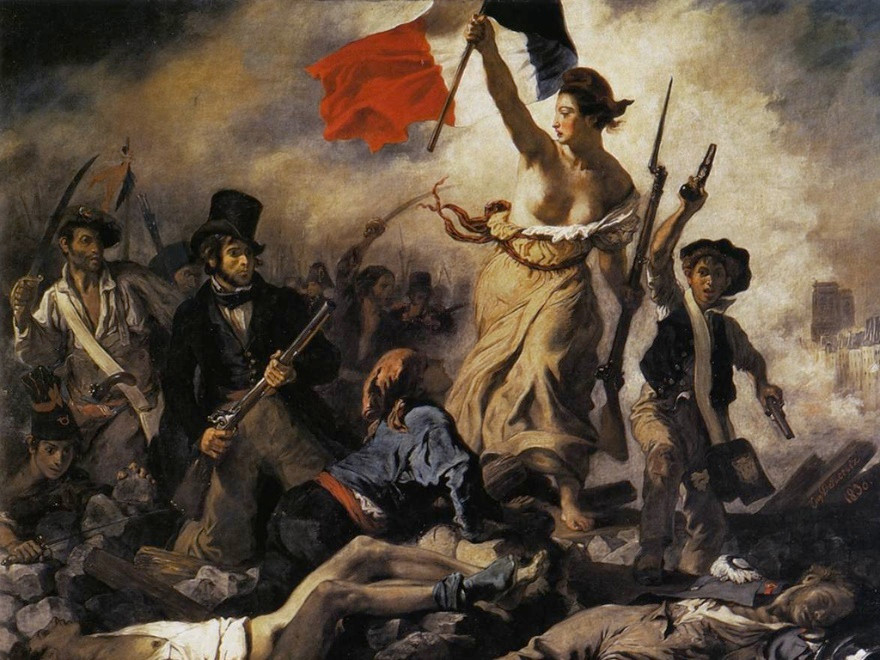
\includegraphics[width=0.6\textwidth]{imagenes/2/libertad-guiando.jpg}
        \caption{Delacroix, \textit{La libertad guiando al pueblo}, 1830}
        \label{fig:libertdad-guiando-pueblo}
    \end{center}
\end{figure}

\subsection{Siglo XX}

Los movimientos de vanguardia vinieron a transformar profundamente y sin retorno a la totalidad de las artes. La arquitectura dejó atrás las formas tradicionales de los historicismos y empezó a hacer uso de los nuevos materiales y tecnologías, además de aumentar su preocupación por el entorno circundante. Aunque tampoco podemos hablar de homogeneidad total, el racionalismo fue la tendencia predominante y la que más impronta dejó en el panorama arquitectónico del siglo XX. Autores como Le Corbusier y Wright levantaron unos edificios ante todo funcionales sirviéndose de líneas puras, formas geométricas y módulos regulares.

En plástica, las vanguardias se manifestaron en lo que ha pasado a la historia como \textit{ismos}. Incontables tendencias de gran originalidad y complejidad teórica coincidieron temporal y espacialmente. Una de las primeras fue el Fauvismo, y su técnica, la más temperamental hasta la fecha, dando todo el protagonismo al color usado de manera emotiva; el Expresionismo, subjetivo y visceral; el Cubismo, rompedor en su visión simultánea de la realidad; el Futurismo y su violencia teórica y expresiva, acorde con el momento histórico del que es fruto; el Surrealismo y su dimensión onírica; y la abstracción en todas sus vertientes, entre otros.

Todas estas corrientes abrieron el camino a un arte definitivamente plural e inclasificable, además de nuevos géneros como la instalación, la \textit{performance} y el arte sonoro, y un sistema de mercado que se ha convertido en el verdadero dueño del devenir artístico.

\subsection{Aplicaciones}

La Historia del Arte ha sido una rama de estudio que siempre ha generado mucho interés, y prueba de ello son las innumerables aplicaciones destinadas a mostrarla de manera didáctica y divulgativa.

En lo que refiere a páginas web existen muchos portales, como \textit{SmartHistory}\footnote{\url{https://smarthistory.org/}} o \textit{The Museum With No Frontiers}\footnote{\url{http://www.museumwnf.org/}}, que proporcionan de manera gratuita y desinteresada toda clase de contenidos y recursos de temática artística.

También, y motivado por la amplia disponibilidad de dispositivos móviles entre la población actualmente, existen diversidad de aplicaciones móvil con este mismo fin, como son \textit{Google Arts \& Culture}\footnote{\url{https://play.google.com/store/apps/details?id=com.google.android.apps.cultural}} que permite a sus usuarios visitar virutalmente exposiciones de arte, o \textit{DailyArt}\footnote{\url{https://play.google.com/store/apps/details?id=com.moiseum.dailyart2}} para Android, que cada día ofrece la imagen y descripción de una obra de arte, ambas también gratuitas.

Y por último, en lo que refiere a videojuegos, se han desarrollado multitud de ellos con temática artística y de museos. Un ejemplo de ello, y en lo que refiere a aventuras gráficas, en 1992 fue lanzado \textit{The Dagger of Amon Ra}, en el que el jugador debe resolver un asesinato en un museo egipcio. Hay muchos más y de muchos otros géneros, como \textit{Discover Babylon}, \textit{Time Explorer} o \textit{Versailles – A game of intrigue at the Court of Louis XIV}.

\section{Realidad Virtual}

Podríamos decir que, en resumen, la Realidad Virtual es una herramienta capaz de crear entornos creíbles, inmersivo e incluso multisensoriales para sus usuarios, de manera que sientan que están en un sitio en el que realmente no están; es decir, se encuentran en un \textbf{mundo virtual}.

Antes de empezar a hablar de la Realidad Virtual, sin embargo, es importante diferenciar los conceptos Realidad Virtual, Realidad Aumentada y Realidad Mixta. Mientras que el primero intenta sumergir por completo al usuario en un mundo virtual, la \textbf{Realidad Aumentada} propone complementar el entorno real superponiendo sobre él objetos digitales. Por último, la \textbf{Realidad Mixta}  une ambos conceptos para permitir interactuar con objetos reales dentro de un mundo virtual, estar completamente inmerso en un mundo virtual o reproducir elementos virtuales en un entorno real.

Los orígenes del concepto de Realidad Virtual no están claros del todo ya que, aplicando la definición anterior, en la época del Renacimiento y con el desarrollo de las técnicas artísticas de perspectiva los propios pintores eran capaces de crear mundos realistas que no existían \cite{schn-17}. 

Sin embargo, las primeras referencias más modernas a este concepto vienen de la mano de un autor de cine. En los años 50 el cineasta \textbf{Morton Heilig} propuso un \textit{experiencia de teatro} con la que poder engañar a los sentidos del  público para transportarles a otro momento y lugar. Pocos años después, en 1962, construyó un prototipo llamado \textbf{Sensorama}, un artilugio capaz de despertar varios de los sentidos de sus usuarios (figura \ref{fig:sensorama}). Este artilugio era capaz de generar en sus usuarios la experiencia de montar en moto en las calles de Brooklin sintiendo el viento en la cara, la vibración del asiento de la motocicleta, una vista tridimensional y los olores de la ciudad. Sin embargo, debido a lo caro que era, no pudo continuarse con su producción \cite{brock-16}.

\vspace{0.2cm}

\begin{figure}[!h]
    \begin{center}
        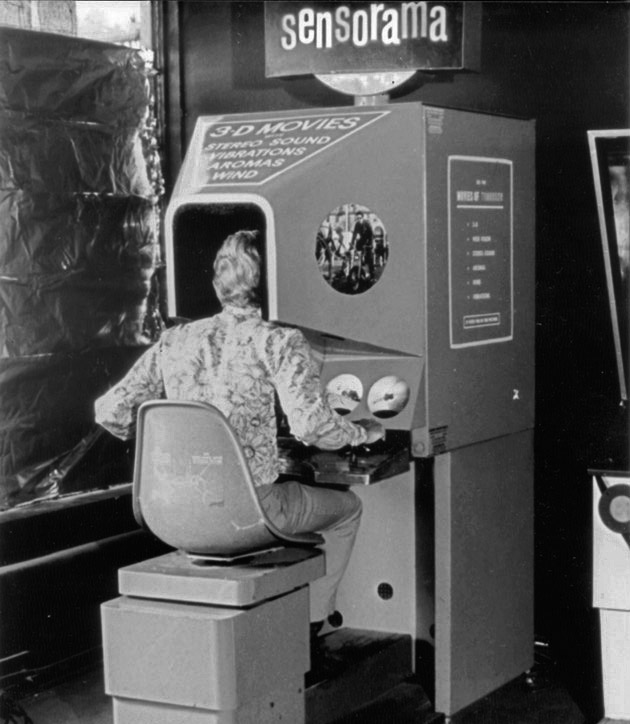
\includegraphics[width=0.5\textwidth]{imagenes/2/sensorama.jpg}
        \caption{Máquina \textit{Sensorama}, \url{www.engadget.com}}
        \label{fig:sensorama}
    \end{center}
\end{figure}

Tres años después, en 1965, el ingeniero \textbf{Ivan Sutherland} escribió el artículo \textit{A head-mounted three dimensional display} \cite{suth-65}, o por sus siglas \acs{HMD}, en el que describe a las imágenes bidimensionales como poco inmersivas y propone un casco con una pequeña pantalla en cada ojo que hacen uso de la \textbf{visión estereoscópica} del ser humano.

Tres años después de la publicación de este artículo, en 1968, Iván Sutherland y su estudiante Bob Sproull desarrollaron el que se considera primer dispositivo para aplicaciones inmersivas. Dado su abultado tamaño, como puede verse en la figura \ref{fig:damocles}, finalmente se le acabó llamando \textbf{\textit{Sword of Damocles}}. Además, este dispositivo contaba con rastreador posicional del casco, por lo que la posición de las imágenes que se visualizaban a través de él correspondía con con su posicionamiento virtual. Pese a todo, y como aún no se disponía de la suficiente tecnología, los gráficos eran muy básicos \cite{lop-18}.

\vspace{0.1cm}

\begin{figure}[!h]
    \begin{center}
        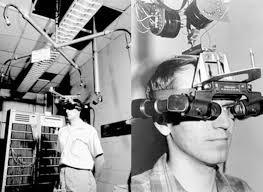
\includegraphics[width=0.6\textwidth]{imagenes/2/damocles.jpg}
        \caption{\textit{Sword of Damocles}, \url{www.dsource.in}}
        \label{fig:damocles}
    \end{center}
\end{figure}

A lo largo de los años setenta, se siguieron desarrollando varios prototipos como \textit{Grope}, de la Universidad de Carolina del Norte, o \textit{Videoplace}, que detectaba mediante cámaras las siluetas de las sombras de los usuarios y las proyectaba sobre una pantalla, lo que les permitía interactuar con ellas \cite{gerv-99}.

Los años 80 fueron muy prolíficos para los simuladores de Realidad Virtual y, paralelamente, comenzaron las primeras discusiones entre diversos filósofos tecnológicos, como Jaron Lanier, Myron Krueger o Ted Nelson, por la búsqueda del término que definiera una tecnología aún en proceso de nacer \cite{lop-18}.

En 1982, Thomas Furnes desarrolló el simulador más avanzado del momento, el \textit{Visually Coupled Airborne Systems Simulator}, o VCASS, que estaba contenido en su totalidad dentro del casco \cite{cade-08}. Aún así seguía siendo bastante voluminoso, como puede verse en la figura \ref{fig:VCASS} 

\begin{figure}[!h]
    \begin{center}
        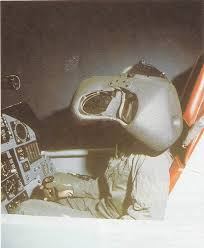
\includegraphics[width=0.4\textwidth]{imagenes/2/VCASS.jpg}
        \caption{\textit{VCASS}, \url{voicesofvr.com}}
        \label{fig:VCASS}
    \end{center}
\end{figure}

Finalmente, el término \textit{Realidad Virtual} fue acuñado por Jaron Lanier, fundador de una de la empresas VPL Research, una de las primeras en comercializar estos sistemas a gran escala \cite{fer-02}. Lanier proponía unos dispositivos que, acoplados en nuestro cuerpo, fueran capaz de hacernos percibir a través de los sentidos sensaciones realistas de un mundo diferente al nuestro, de tal manera que cuanto más avanzados sean estos dispositivos más realistas serán las sensaciones y más difícil será diferenciar entre este mundo y el real \cite{lop-18}.

Y poco a poco, principalmente movido por la creciente industria del videojuego y sus múltiples usos potenciales, estas tecnologías han seguido desarrollándose. Una de las primeras aplicaciones comerciales en los videojuegos fue la \textit{Virtual Boy} de Nintendo. Fue lanzada al mercado en 1995 y contaba con dos pequeñas pantallas monocromáticas que reproducían juegos. Este dispositivo puede verse en la figura \ref{fig:virtual-boy}.

\begin{figure}[!h]
    \begin{center}
        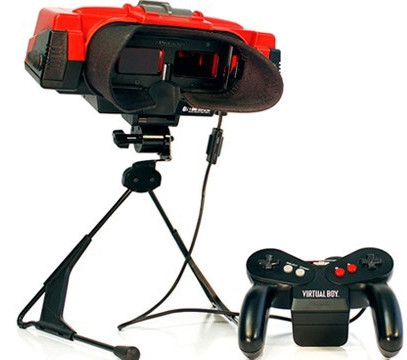
\includegraphics[width=0.45\textwidth]{imagenes/2/virtual-boy.jpg}
        \caption{\textit{Virtual Boy}, \url{codigoespagueti.com}}
        \label{fig:virtual-boy}
    \end{center}
\end{figure}

Aunque esta consola fue un fracaso (apenas se vendieron 770.000 unidades en todo el mundo\footnote{\url{http://www.gamepro.com/gamepro/domestic/games/features/111823.shtml}, 2007}) demostró que se podían desarrollar dispositivos similares.

Y con esto llegamos a la actualidad, donde poco a poco, y principalmente por el abaratamiento de esta tecnología, el mercado de dispositivos de Realidad Virtual está creciendo y cada vez hay más dispositivos al alcance de los usuarios.

\subsection{Dispositivos}

Actualmente, los principales dispositivos que permiten jugar en \acs{VR} destinados a usuarios normales y que, por tanto, son en los que se ha centrado este \acs{TFM}, son los siguientes.

\subsubsection{Oculus Rift} 

En el año 2012, Palmer Lucky fundó la compañía Oculus VR con la idea de crear un dispositivo destinado a jugar en \acs{VR} y con un precio viable para los jugadores casuales. A finales de ese mismo año, y con ayuda de John Carmack (programador en juegos como Doom, Quake o Wolfenstein), mostró el primer prototipo del dispositivo y fue un éxito, por lo que lanzó una campaña en Kickstarter que superó con creces el dinero necesario, consiguiendo caso 2 millones y medio de dólares\footnote{\url{https://www.kickstarter.com/projects/1523379957/oculus-rift-step-into-the-game}} y que puede verse en la figura \ref{fig:oculus}.
    
\begin{figure}[!h]
\begin{center}
    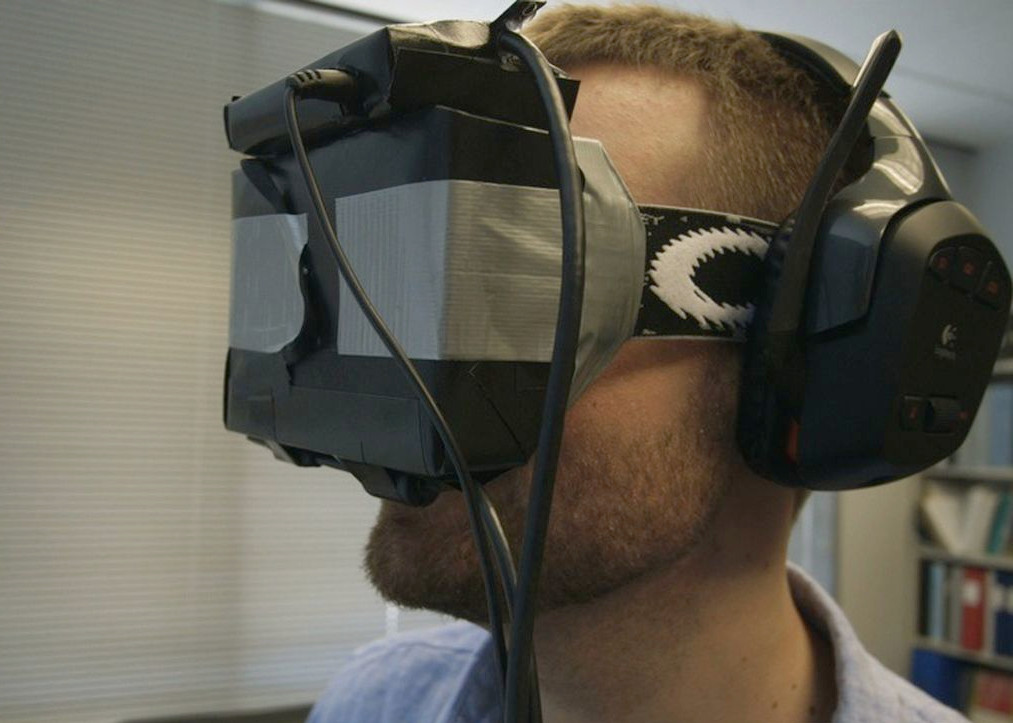
\includegraphics[width=0.5\textwidth]{imagenes/2/oculus-prototipo.jpg}
    \caption{Prototipo del \textit{Oculus Rift}, \url{www.theverge.com}}
    \label{fig:oculus}
\end{center}
\end{figure}

Año tras año fue mejorando sus prototipos hasta que en marzo de 2014 Facebook compró esta compañía por un total de 2,300 millones de dólares. Finalmente, en mayo de 2015, se anunció la versión finalizada de las gafas lista para su comercialización. Actualmente pueden comprarse por unos 240\euro.

\subsubsection{HTC Vive} 

Vive son unas gafas de realidad virtual co-fabricadas por HTC y Valve. En 2014 se mostraron los primeros prototipos de un sistema de realidad virtual producido por la empresa Valve, pero no fue hasta marzo de 2015 cuando HTC reveló oficialmente las Vive. Antes de la versión para consumidores se fabricaron las Vive PRE, que fueron gratuitas para algunos desarrolladores de videojuegos con el fin de promover sus aplicaciones. 

\begin{figure}[!h]
\begin{center}
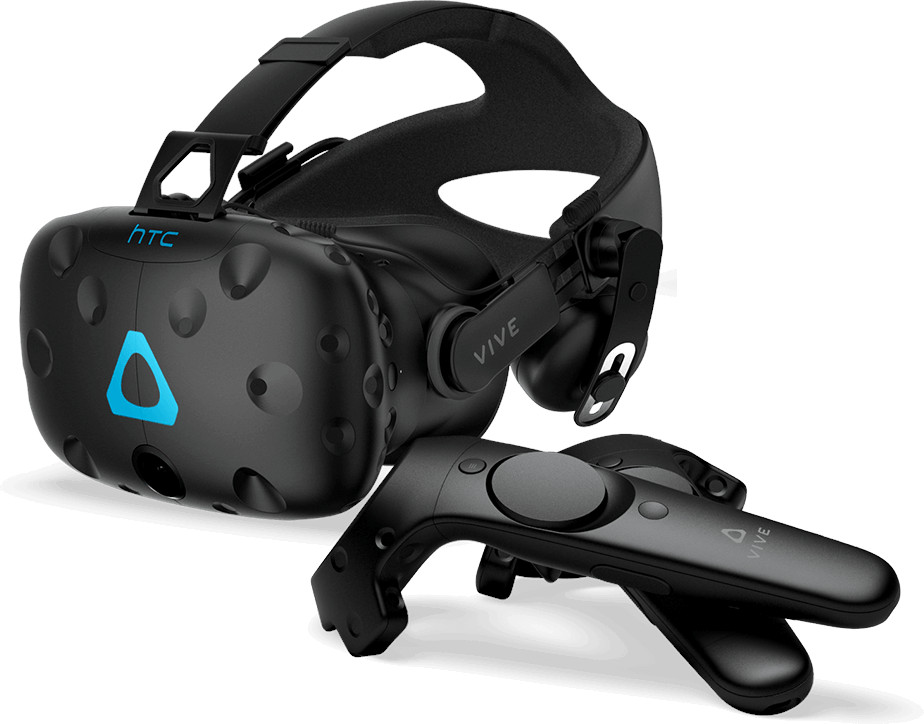
\includegraphics[width=0.5\textwidth]{imagenes/2/htc-vive.jpg}
\caption{HTC Vive}
\label{fig:htc-vive}
\end{center}
\end{figure}

A principios de 2016 se anunció su lanzamiento con un precio de salida de 900\euro, aunque actualmente pueden adquirirse por la mitad, unos 450\euro.

\subsubsection{PlayStation VR} 

Este headset no es la primera propuesta de PlayStation de \acs{VR}. Su primer intento comercial, \textit{Glasstron}, se lanzó en 1997 para el juego \textit{MechWarrior 2}. Estas gafas permitían a jugadores adoptar una perspectiva visual desde dentro de la cabina de la nave, como si la controlaran.

\vspace{0.1cm}

\begin{figure}[!h]
\begin{center}
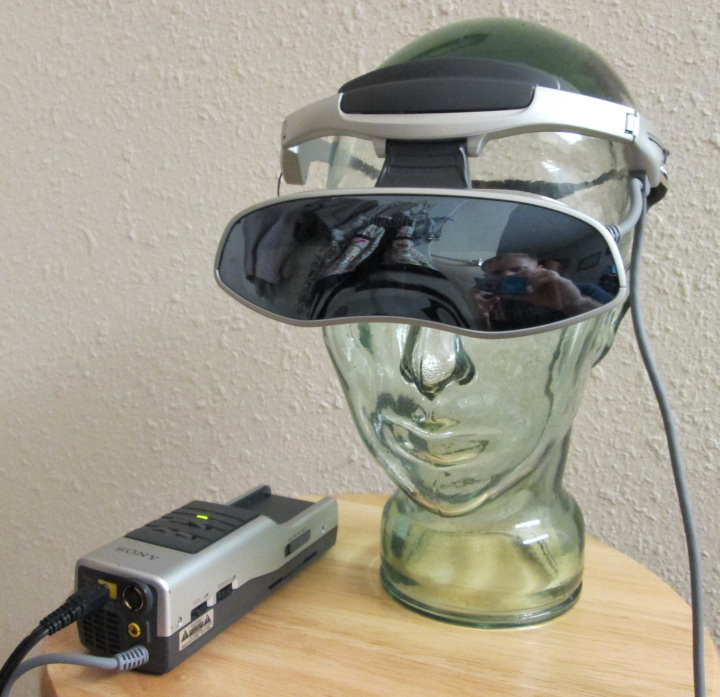
\includegraphics[width=0.5\textwidth]{imagenes/2/glasstron.jpg}
\caption{Gafas \textit{Glasstron}, \url{http://www.mellottsvrpage.com}}
\label{fig:glasstron}
\end{center}
\end{figure}

A mediados de 2014, el desarrollador de PlayStation Anton Mikhailov anunció en una conferencia que su equipo había estado trabajando en el Project Morpheus durante 3 años, rediseñando el \textit{PlayStation Move} para adaptarlo a la tecnología \acs{VR}. Al año siguiente este proyecto se bautizó como \textit{PlayStation VR}. Finalmente lanzada al mercado en 2016, actualmente puede comprarse por unos 250\euro, aunque solo funciona con un sistema PlayStation 4.
    
\subsubsection{Lenovo Explorer} 

La compañía Lenovo también ha dado el salto a los headsets \acs{VR} desarrollando uno propio, llamado Explorer. Este dispositivo, lanzado al mercado en octubre de 2017, hace uso del \textit{Microsoft Mixed Reality}, un framework de desarrollo implementado por Microsoft para su headset \acs{AR}, las \textit{Microsoft HoloLens}. Como su nombre sugiere, este framework está pensado para trabajar tanto con tecnologías \acs{VR} como \acs{AR}.
    
A diferencia del resto de headsets, el Explorer tiene dos pequeñas cámaras integrados en la parte delantera, lo que le permite escanear y transmitir la ubicación del usuario, de los mandos y del entorno haciendo uso de la tecnología de rastreo sin balizas de Microsoft, similares a las que se usan para HoloLens. Además incluye dos controladores, como puede verse en la figura \ref{fig:lenovo-explorer}.

\begin{figure}[!h]
\begin{center}
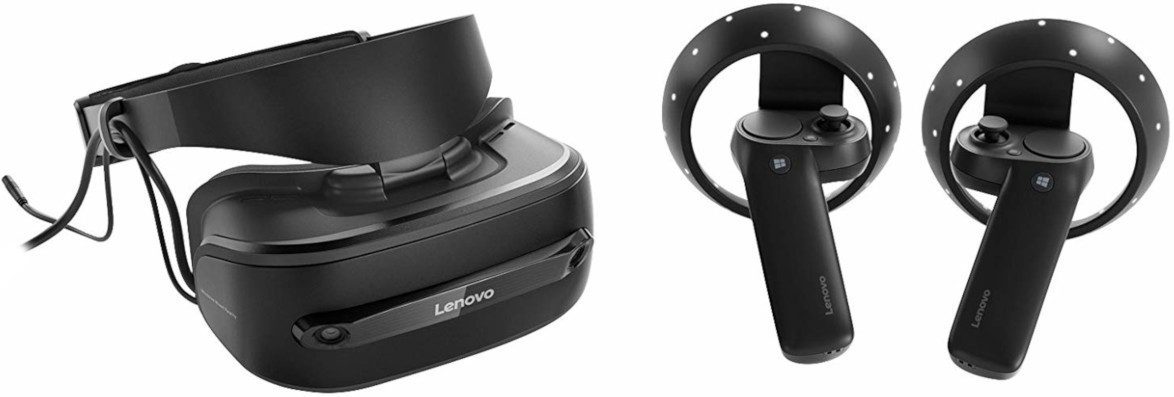
\includegraphics[width=0.8\textwidth]{imagenes/2/lenovo-explorer.jpg}
\caption{Gafas \textit{Lenovo Explorer}}
\label{fig:lenovo-explorer}
\end{center}
\end{figure}

Además, tienen el precio más competitivo de todas, llegando a haber podido ser compradas en la página \url{pccomponentes.com} por 150\euro, como puede verse en la figura \ref{fig:precios-explorer}, aunque actualmente ronde los 200\euro. 

\begin{figure}[!h]
\begin{center}
    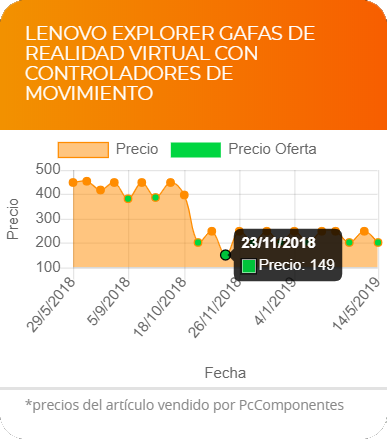
\includegraphics[width=0.4\textwidth]{imagenes/2/precios-explorer.png}
    \caption{Historial de precios de las Lenovo Explorer, \url{pccomponentes.com}}
    \label{fig:precios-explorer}
\end{center}
\end{figure}

Por todo esto se cree que son las más probables para ser adquiridas en los jugadores interesados en esta tecnología, por lo que han sido elegidas para usarse en este proyecto. En el capítulo \ref{chap:tecnologia} se hablará en más profundidad de su tecnología y sus especificaciones técnicas.

\subsubsection{Google Cardboard} 

La opción más económica para comenzar en el mundo de la \acs{VR} son los headsets de cartón. El más famoso es el de Google, que permite usar un teléfono móvil como pantalla para abaratar mucho los costes, de manera que el headset es simplemente una caja de cartón vacía con dos pequeñas lentes para los ojos, como puede verse en la figura \ref{fig:google-cardboard}, y que puede comprarse en Amazon por menos de 10\euro.
    
\begin{figure}[!h]
\begin{center}
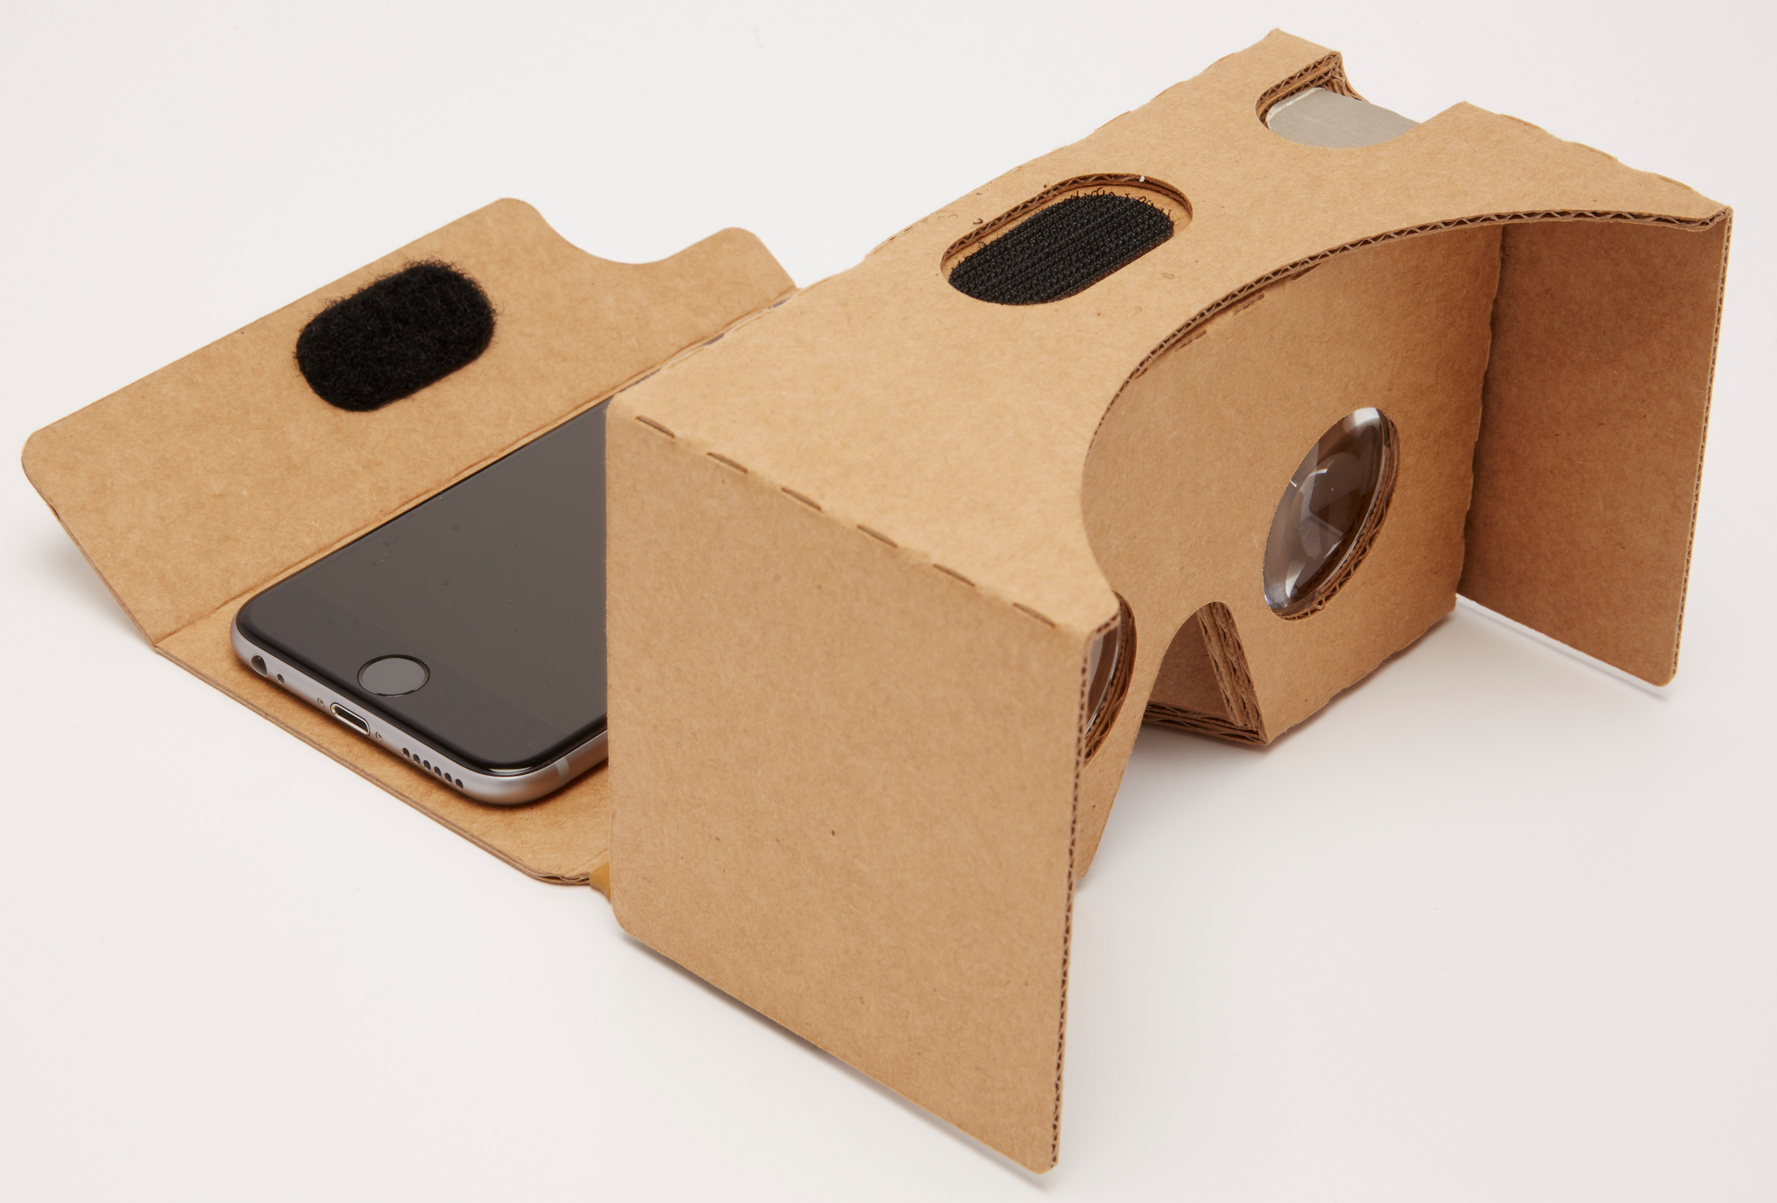
\includegraphics[width=0.5\textwidth]{imagenes/2/cardboard.jpg}
\caption{Google Cardboard abiertas}
\label{fig:google-cardboard}
\end{center}
\end{figure}

El principal problema es que los móviles, al no ser dispositivos especialmente potentes, no permiten el renderizado de escenarios complejos, por lo que no consiguen una sensación de inmersión muy buena.

\subsubsection{Index VR}

Anunciado por Valve en mayo de este año y aún no disponible para comprar, Index VR\footnote{\url{https://www.valvesoftware.com/es/index}} es el último headset incluido en la lista. Es un dispositivo para jugar en \acs{VR} compuesto por un headset, dos controladores y dos estaciones de posicionamiento (figura \ref{fig:index-vr}) que, según la propia Valve, permitirán un \textit{tracking} mucho más preciso de la posición y los movimientos de los jugadores, que podrán moverse libremente en un área de 10x10 metros.

\begin{figure}[!h]
\begin{center}
    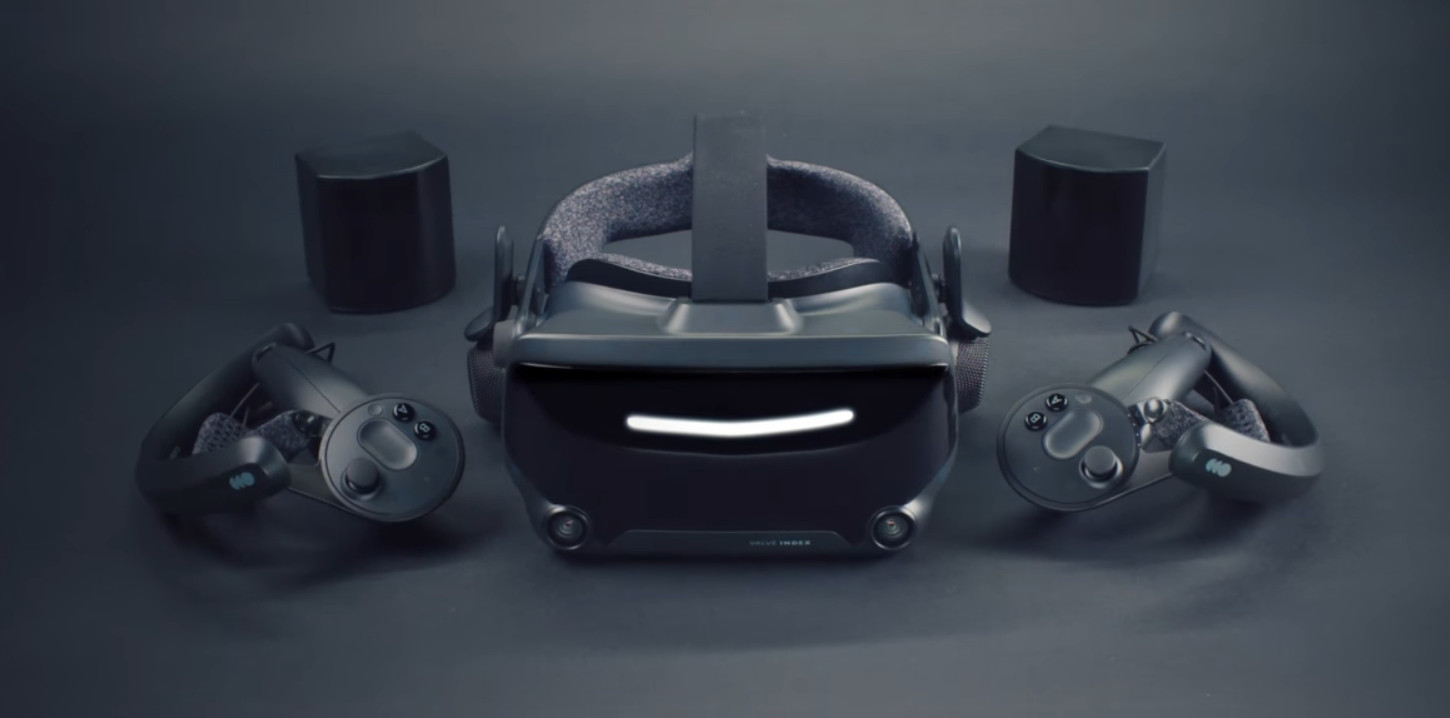
\includegraphics[width=0.85\textwidth]{imagenes/2/indexvr.jpg}
    \caption{\textit{IndexVR} de Valve}
    \label{fig:index-vr}
\end{center}
\end{figure}

Por otro lado, es de lejos el dispositivo destinado al público general más caro del mercado, estando disponible para reserva el pack con los tres periféricos anteriormente presentados por 1080\euro.

\subsection{Librerías de desarrollo}

Como la Realidad Virtual es una tecnología relativamente nueva que aún no se ha abaratado todo lo que puede, no ha conseguido llegar a los hogares de la mayoría de sus potenciales usuarios. Por tanto, como la demanda es muy baja, la oferta de aplicaciones también lo es y, en consecuencia, hay muy pocas empresas que hayan invertido en desarrollar frameworks y librerías de desarrollo para aplicaciones que hagan uso de la Realidad Virtual.

Aún así, han aparecido algunas librerías desarrollados por empresas con la mayor cuota de mercado y que pueden permitirse innovar, como Steam, y otras que se han centrado en esta tecnología y lo necesitaban, como Oculus. A continuación se presentan las más importantes.

\subsubsection{VRTK}

\acl{VRTK}\footnote{\url{https://vrtoolkit.readme.io}} es un framework de desarrollo multi-librería desarrollado en solitario bajo licencia \acs{MIT} por \textit{TheStoneFox}\footnote{\url{https://github.com/thestonefox}}, o Harvey Ball, un hombre residente en Birmingham, Reino Unido. Este framework solo está disponible para el \acs{IDE} Unity3D y permite desarrollar paralelamente para distintas librerías a través de una interfaz común; es decir, podemos desarrollar para SteamVR y Oculus a la vez usando la interfaz de \acs{VRTK}.

Pero el desarrollo de esta librería no ha sido fácil para \textit{TheStoneFox}; todo empezó en abril de 2016 cuando, sin apenas experiencia en desarrollo de videojuegos, comenzó un proyecto con Unity3D y SteamVR y se dio cuenta de lo confuso y poco documentado que estaba todo, por lo que decidió desarrollar su propio \acs{SDK} o, en sus propias palabras\footnote{\url{https://uploadvr.com/vrtk-stone-fox-unity-tool/}},

\begin{displayquote}
\textit{I wanted to build something for it as I was new to game dev. I’d been using Unity for about a month just as a hobby, I tried to use the SteamVR Unity plugin and found it confusing, realized a lot of people found it confusing and started VRTK as a way to help people get into developing for VR."}
\end{displayquote}

Y poco a poco fue avanzando en su proyecto y ganando la atención de los desarrolladores hasta que decidió abrirse una cuenta de Patreon\footnote{\url{https://www.patreon.com/vrtk}}, donde llegó a ingresar 2000\$ al mes, y lo que comenzó como un pasatiempo a tiempo parcial se conviritó en su único proyecto. Además, comenzó a realizar conferencias por todo el mundo gracias a las que fue ganando popularidad, como la \textit{Unite Europe 2017}, cuya ponencia puede verse en YouTube\footnote{\url{https://youtu.be/AbIiBrg8yT4}}.

Pero a finales de 2017, entre el nulo apoyo que recibía de la comunidad, que hacía que él fuera literalmente el único desarrollador del proyecto (como puede verse en la figura \ref{fig:stonefox-twitter}), y que no quería que la cuenta de Patreon diera la impresión de que el proyecto era solvente, porque no lo era, decidió cerrar esta cuenta y dar por finalizado el proyecto. Aún así, aunque dijo que no añadiría funcionalidad nueva, se comprometió a seguir manteniéndolo durante algún tiempo, principalmente arreglando bugs\footnote{\url{https://skarredghost.com/2017/12/28/vrtk-shutting-will-make-vr-development-unity-easier-now/}}.

\begin{figure}[!h]
\begin{center}
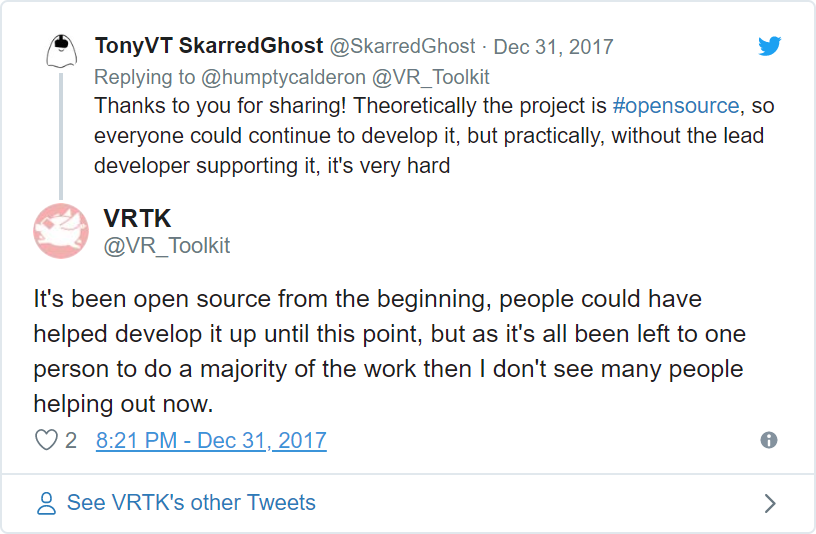
\includegraphics[width=0.8\textwidth]{imagenes/2/stonefox-twitter.png}
\caption{\textit{TheStoneFox} en Twitter sobre los motivos del cierre de \acs{VRTK}}
\label{fig:stonefox-twitter}
\end{center}
\end{figure}

Por suerte, cuatro meses después y gracias a una donación por parte de Oculus, el proyecto volvió a la vida. El propio \textit{TheStoneFox} aclaraba en Twitter que no era ningún tipo de compra, ya que \acs{VRTK} seguiría siendo gratuito y mantendría la misma filosofía que antes de cerrarse\footnote{\url{https://skarredghost.com/2018/04/30/vrtk-announces-version-4-thanks-to-an-oculus-grant/}}.

A día de hoy la página de Patreon vuelve a estar abierta, aunque apenas ingresa un tercio de la cantidad de antes de dar por finalizado el proyecto.

Actualmente existen varios proyectos comercializados desarrollados gracias a este framework, como \textit{Deism}, \textit{One of the last} u \textit{Oddescape}. Uno de los más famosos es \textit{quiVr}\footnote{\url{http://quivr.net/}}, un \textit{tower defense} en el que el jugador encarna a un arquero que debe acabar con todas las oleadas de enemigos que aparecen antes de que lleguen a su base.

\textit{TheStoneFox} también realiza pequeños vídeos enseñando todos los juegos que utilizan su framework con el fin de darles publicidad y de mostrar la potencia que tiene. Todos estos vídeos pueden verse en una lista de reproducción\footnote{\url{http://yt.vu/p/PLTiD-q2AfVNIrAN5w0WK6hOyjy6zL1tWv}} en la que los añade. 

\subsubsection{SteamVR}

Steam es una plataforma de distribución digital de videojuegos cuya dueña es Valve. Steam lanzó en 2014 una nueva iniciativa para adaptar la Realidad Virtual a los juegos digitales, llamada SteamVR\footnote{\url{https://steamcommunity.com/steamvr}}, que permite el desarrollo y uso de juegos de realidad virtual a partir de su plataforma, es decir, solo los juegos distribuidos en Steam podrán acceder a estas librerías.

A principios de  2014, Valve inició un proyecto para \acs{VR} para su plataforma. En junio de 2014 se mostraron los primeros avances pero no fue hasta la Mobile World Congress de 2015 cuando se anunció públicamente. El primer dispositivo que usó esta tecnología fue el HTC Vive, el headset \acs{VR} de HTC.

Actualmente la plataforma cuenta con más de 1200 experiencias \acs{VR} con todo tipo de juegos y simuladores. Además, desde 2017 tienen en fases de desarrollo la incorporación de la Realidad Aumentada en colaboración con Microsoft\footnote{\url{https://generacionxbox.com/microsoft-steamvr-realidad-aumentada/}}.

\subsubsection{Windows Mixed Reality}

Windows Mixed Reality, anteriormente Windows Holographic, es una plataforma de \acs{MR} desarrollada por Microsoft e incluida de manera nativa en Windows 10 desde principios de 2018.

El principal dispositivo para este framework son las Microsoft HoloLens, un headset que en realidad es un ordenador inalámbrico autónomo corriendo Windows 10. Utiliza sensores avanzados, dos pantallas estereoscópicas de alta definición y sonido espacial que le permiten ejecutar aplicaciones de realidad aumentada.

Las HoloLens estuvieron desarrollándose durante casi cinco años antes de su lanzamiento público en 2015, aunque inicialmente fue concebido no como un headset independiente sino como una tecnología para la cámara Kinect\footnote{\url{https://www.wired.com/2015/01/microsoft-hands-on/}}.

Inicialmente, las HoloLenses únicamente estaban disponibles en Norteamérica, pero gracias a la positiva respuesta que han recibido de parte de sus usuarios llegarán próximamente a Europa.

Además, con el fin de atraer a más usuarios, Microsoft ha lanzado \textbf{Windows Mixed Reality for SteamVR}, un wrapper que permite jugar a juegos desarrollados con la librería SteamVR con un headset que implemente su tecnología. Es necesario descargar este software desde Steam como si fuera un juego.

\subsubsection{Oculus SDK}

El framework de desarrollo para Oculus, también llamado Oculus SDK\footnote{\url{https://developer.oculus.com/downloads/}}, es un conjunto de librerías desarrolladas por Oculus para su headset \acs{VR}, Oculus Rift.

Este \acs{SDK} está disponible para los IDEs Unity3D y Unreal Engine, además de poder descargarse para trabajar directamente en Windows.
    

\subsection{Aplicaciones}

Los usos de la tecnología \acs{VR} son casi tan variados como los colectivos la utilizan. En esta sección se presentan las principales aplicaciones de la \acs{VR}.

\subsubsection{Simulación}

Una de las aplicaciones más potentes de la \acs{VR} es la simulación. Por su componente inmersivo, la \acs{VR} es perfecta para este tipo de aplicaciones, ya que permite a sus usuarios sentir que están en un entorno diferente sin los peligros que pueda conllevar.

Dentro de la simulación, uno de los campos de aplicación más importantes es el militar, donde poder entrenar a personas para situaciones de riesgo sin poner en peligro sus vidas es de vital importancia.

Un ejemplo de esto es el Departamento de Defensa de los Estados Unidos de América, que ha desarrollado el \textit{Weapons Augmented Reality Scoring System}, o WARSS, un entorno en el que los soldados pueden practicar situaciones y tácticas a las que podrían enfrentarse un día usando tecnologías \acs{VR} y \acs{MR}, concretamente con dispositivo HoloLens de Microsoft, como puede verse en la figura \ref{fig:warss}.

\begin{figure}[!h]
\begin{center}
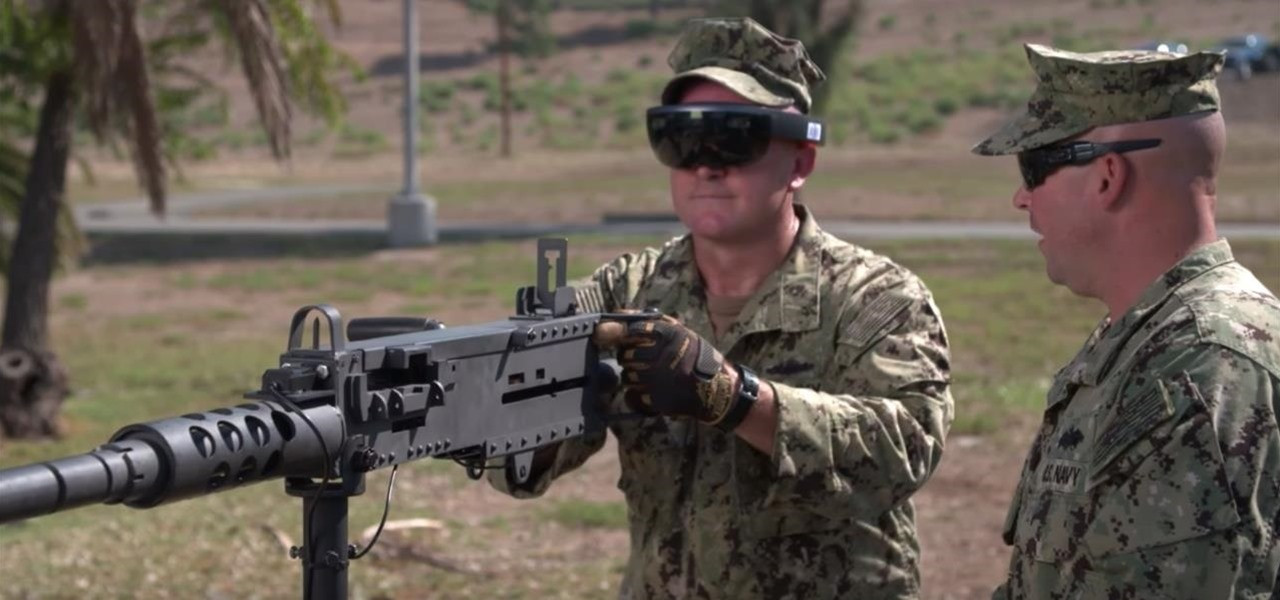
\includegraphics[width=0.8\textwidth]{imagenes/2/WARSS.jpg}
\caption{Soldados del ejército americano haciendo uso de la tecnología WARSS, \url{https://hololens.reality.news}}
\label{fig:warss}
\end{center}
\end{figure}

Otro de los campos en los que triunfa esta tecnología por los mismos motivos es en la la medicina, donde es imprescindible que los médicos sepan cómo manejar situaciones delicadas para la vida de los pacientes antes de tener que enfrentarse a ellas por primera vez ya que, gracias a la ayuda de programadores y modeladores 3D, se puede reproducir con exactitud la anatomía de los pacientes y practicar crujías antes incluso de llevarlas a cabo, reduciendo los costes de utilización de cadáveres para pruebas y permitiendo repetir la operación cuantas veces fuera necesario.

En figura \ref{fig:medico} puede verse a un cirujano con el headset \acs{VR} Oculus Rift haciendo uso de esta tecnología.

\begin{figure}[!h]
\begin{center}
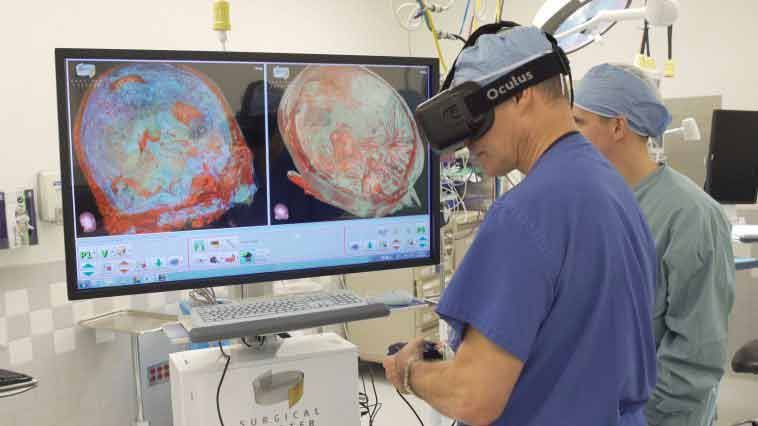
\includegraphics[width=0.8\textwidth]{imagenes/2/medicina.jpg}
\caption{Médico simulando una operación, \url{http://www.baboonlab.com}}
\label{fig:medico}
\end{center}
\end{figure}
 
\subsubsection{Videojuegos}

Como ya se ha expuesto antes, la industria de los videojuegos es actualmente una de las más lucrativas y, como los propios videojuegos requieren de la inmersión de sus usuarios, ha sido fácil para la \acs{VR} abrirse paso a través de ella.

Actualmente, los juegos en \acs{VR} que más éxito tienen en Steam\footnote{\url{https://store.steampowered.com/vr/}} son aquellos en los que el jugador debe disparar, ya sea con armas, como en el caso de \textit{Pavlov VR} o \textit{Blade and Sorcery}, o con arcos, como en \textit{Elven Assassin}, como puede verse en la figura \ref{fig:elven-assassin}.

\begin{figure}[!h]
\begin{center}
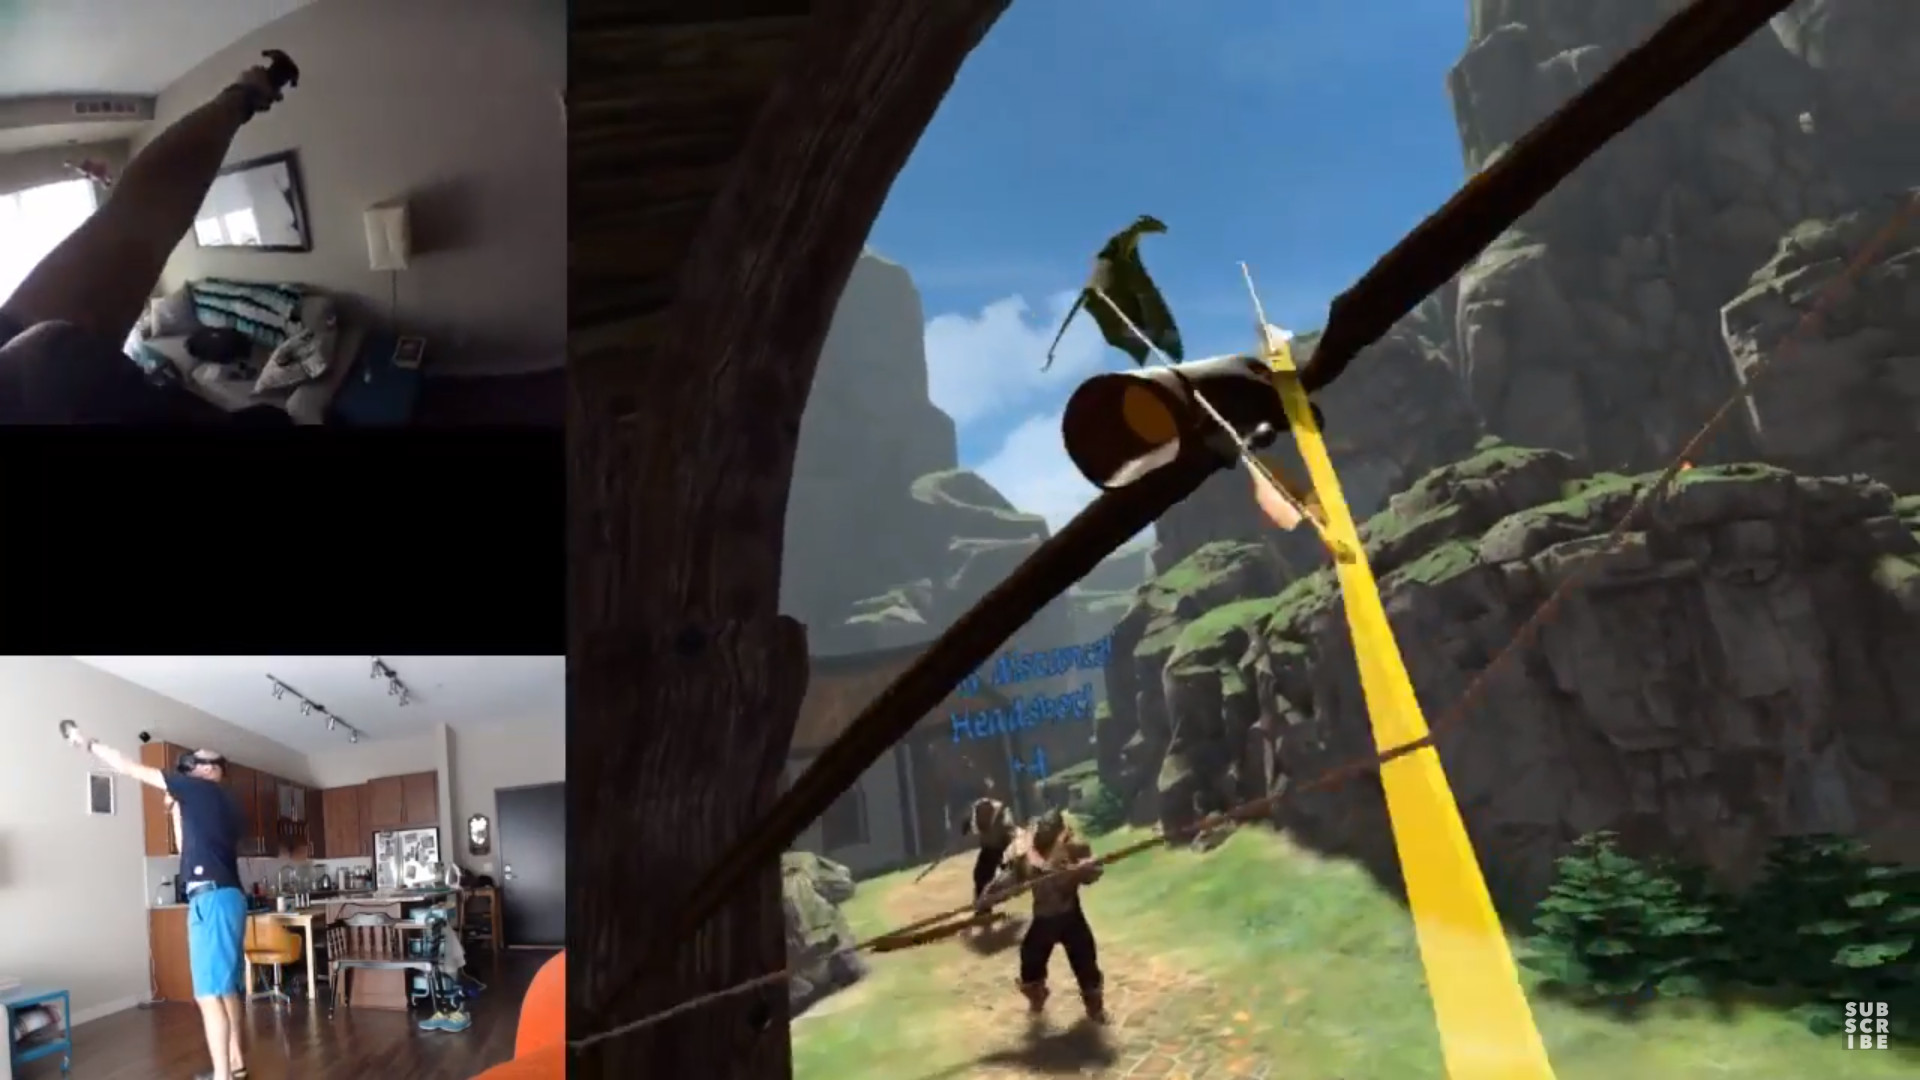
\includegraphics[width=0.7\textwidth]{imagenes/2/elven-assassin.jpg}
\caption{Elven Assassin, \textit{YouTube/BenPlaysVR}}
\label{fig:elven-assassin}
\end{center}
\end{figure}

\subsubsection{Reconstrucción}

Dada la naturaleza inmersiva de la \acs{VR}, es perfecta para, mediante sistemas de modelado tridimensionales, recrear lugares tal y como eran en algún momento de la historia para poder estudiarlos o verlos fácilmente.

Un ejemplo de esto sería las aplicaciones \acs{VR}\footnote{\url{https://uploadvr.com/notre-dame-vr/}} que han surgido a raíz de la cercana trajeada que sufrió la iglesia de Notre-Dame de París en la que un incendio provocó que la mayor parte de su interior se quemara. Estas aplicaciones permiten ver cómo era antes del incendio de un modo mucho más realista e inmersivo que verlo a través de un vídeo.

\section{Diseño 3D}

El diseño 3D es esencial en el desarrollo de \MineRVa, ya que tanto a la hora de diseñar y modelar las salas como implementar sus funcionalidades será necesario basarse en este área.

En esta sección se presentarán y describirán las dos áreas del diseño 3D más importantes para desarrollo de este proyecto.

\subsection{Suites de modelado 3D}

Lo principal a la hora de trabajar con modelos 3D es poder diseñarlos y modelarlos, Para ello, actualmente existen multitud de programas y suites completas a disposición de los usuarios. Los más importantes y con la mayor cuota de mercado son los siguientes. 

\subsubsection{Blender}

Blender\footnote{\url{https://www.blender.org/}} es un programa informático multiplataforma, dedicado especialmente al modelado, iluminación, animación y renderizado de gráficos tridimensionales, además de incluir herramientas para esculpir tridimensionalmente y hasta un motor de juegos propio, el Blender Game Engine. Aunque inicialmente era distribuido de forma gratuita pero sin el código fuente, actualmente es \textit{open source} bajo la licencia GNU General Public License, o GPL, y está disponible para prácticamente todos los sistemas operativos para ordenador.

\begin{figure}[!h]
\begin{center}
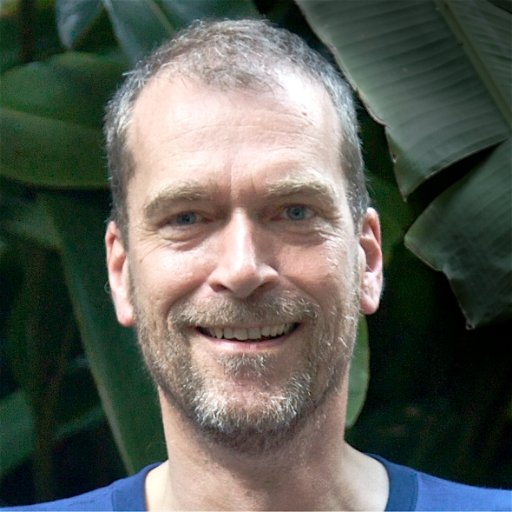
\includegraphics[width=0.4\textwidth]{imagenes/2/roosendaal.jpg}
\caption{Tom Roosendaal, imagen obtenida de su cuenta de Twitter}
\label{fig:roosendaal}
\end{center}
\end{figure}

Todo empezó a finales de los años 80 cuando Ton Roosendaal, el futuro fundador de Blender, era el líder de NeoGeo, el mayor estudio de animación de Holanda. Por aquel entonces la herramienta 3D que utilizaban era muy lenta y cara de mantener, por lo que decidieron reescribirla de 0, plantando la semilla de lo que después sería el software de creación que ahora conocemos como Blender\footnote{\url{https://www.blender.org/foundation/history/}}. 

Pero mientras que NeoGeo continuaba trabajando en Blender, Roosendaal pensó que el mundo entero podría beneficiarse de su herramienta, por lo que a finales de los 90 fundó una división de NeoGeo, Not a Number (o NaN a partir de ahora) para distribuir gratuitamente Blender y fomentar su desarrollo y su mercado, ya que la mayoría de los programas comerciales de modelado de la época costaban miles de dólares.

A principios del año 2000, NaN recaudó más de 4,5 millones de euros procedente de sus inversores, y pronto pasó a tener más de 50 empleados trabajando alrededor del mundo intentando mejorar y promocionar Blender, publicando la versión 2.0 unos meses después.

Desafortunadamente, debido a las decepcionantes ventas y al continuo clima de dificultades económicas, los inversores decidieron dar por terminado el desarrollo de Blender. Pero por suerte Roosendaal no permitió que Blender desapareciera, así que en marzo de 2002 fundó la organización no lucrativa Blender Foundation, cuyo primer objetivo fue continuar con el desarrollo como un proyecto de código abierto basado en la comunidad de usuarios.

La compañía tuvo que obtener 100,000\euro \ para poder comprar los derechos del código fuente y los de propiedad intelectual de Blender a su antigua compañía, NaN, que consiguieron ser reunidos por la comunidad en menos de 7 semanas. Finalmente, el 13 de octubre de 2002, Blender fue liberado al mundo bajo los términos de GNU General Public License. 

Actualmente, el desarrollo de Blender sigue gracias a un equipo de voluntarios procedentes de diversas partes del mundo, liderados por Ton Roosendaal, que continúan actualizándolo gracias a las donaciones en su página web, obteniendo actualmente 36,521\euro \ al mes\footnote{\url{https://fund.blender.org/}}. Además, periódicamente realizan cortos en los que muestran la potencia de su herramienta como \textit{Big Buck Bunny}, \textit{Caminandes}, \textit{Sintel} o \textit{Agent 327}.

\begin{figure}[!h]
\vspace{0.5cm}
\begin{center}
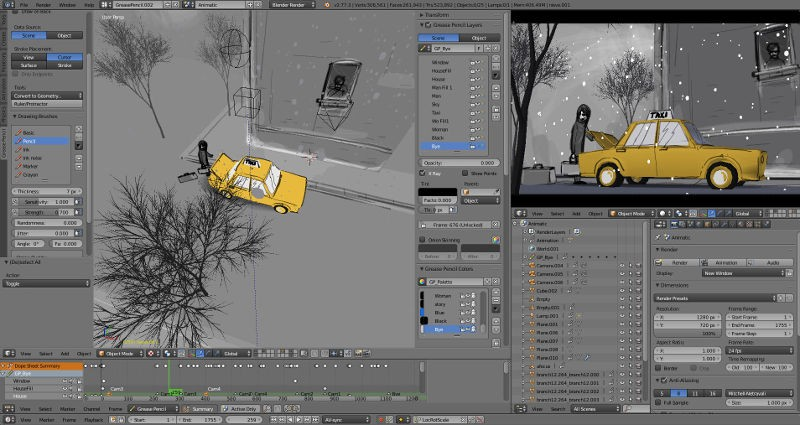
\includegraphics[width=0.9\textwidth]{imagenes/2/blender.jpg}
\caption{Captura de pantalla del entorno de trabajo de Blender}
\label{fig:blender}
\end{center}
\vspace{-0.5cm}
\end{figure}

\subsubsection{Autodesk Maya}

Maya es un programa informático dedicado al desarrollo de gráficos 3D por ordenador, efectos especiales y animación. Además, es el único software de 3D acreditado con un Oscar gracias al enorme impacto que ha tenido en la industria cinematográfica como herramienta de efectos visuales.

Maya surgió tras la fusión de Alias y Wavefront, dos empresas canadienses dedicadas al \acs{CGI} los gráficos generados por ordenador, ya que ambas se utilizaban de manera conjunta prácticamente siempre. Este programa se desarrolló en estrecha colaboración con Disney durante la producción de Dinosaurio a finales de la década de los 1990. Una de los requisitos de Disney era que la interfaz gráfica de usuario pudiera ser fácilmente personalizable, lo que ayudó a que años después Maya se convirtiera en el estándar de la industria gracias a que cada compañía podía cambiar la \acs{GUI} a su gusto.

Autodesk Maya se comercializaba en dos versiones; \textit{Maya Complete} es la versión básica y \textit{Maya Unlimited} la avanzada, que contiene a su versión más simple además de añadir toda clase de módulos con funcionalidad para trabajar con pelo, tejidos, fluidos\dots{}.

\begin{figure}[!h]
\begin{center}
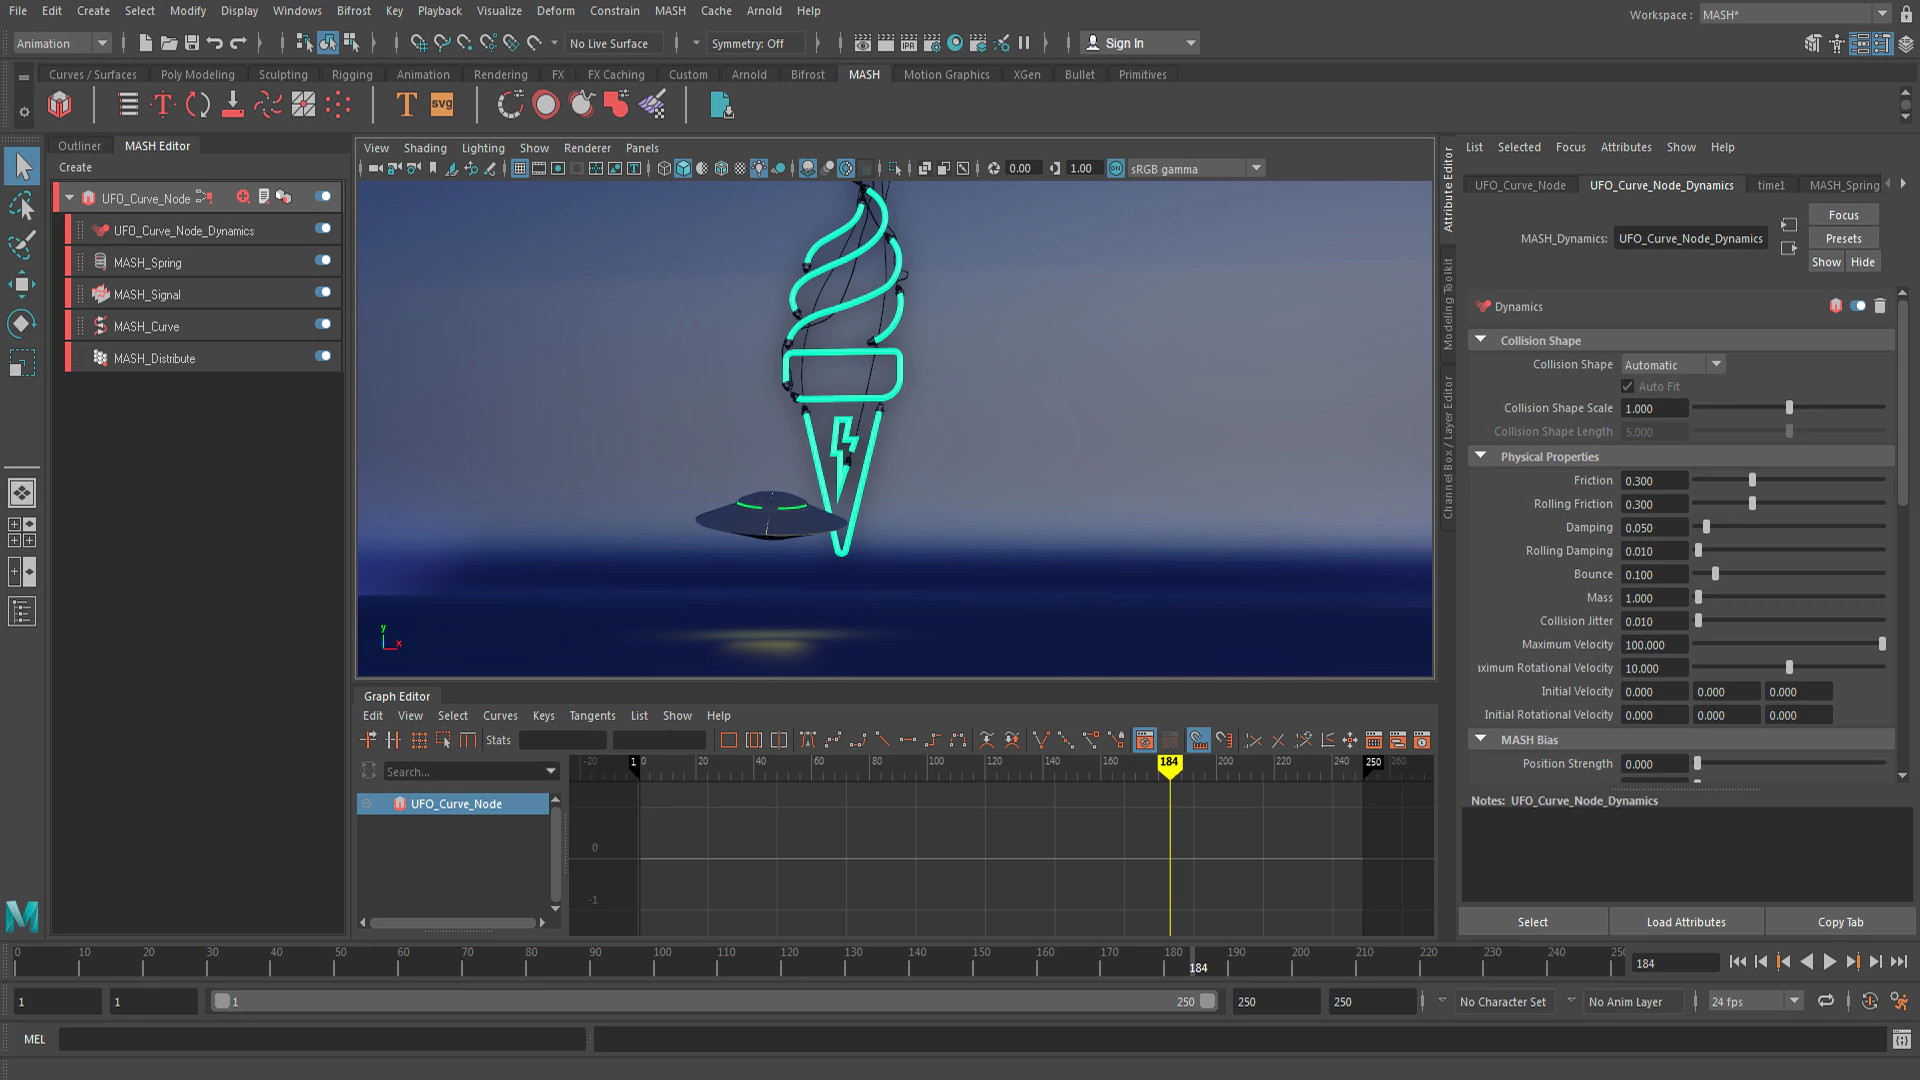
\includegraphics[width=0.9\textwidth]{imagenes/2/maya.jpg}
\caption{Captura de pantalla del entorno de trabajo de Maya}
\label{fig:maya}
\end{center}
\end{figure}

\subsubsection{Autodesk 3Ds Max}

Anteriormente 3D Studio Max, Autodesk 3Ds Max es un programa de creación de gráficos y animación 3D desarrollado por Autodesk, que lo compró a su anterior dueño por 182 millones de dólares. Actualmente es uno de los programas de animación 3D más utilizado, especialmente para el desarrollo de videojuegos, anuncios de televisión y arquitectura.

Todo empieza a mediados de los años 1980, con la creación del Grupo Yost. Este grupo estaba compuesto por varios expertos del sector que comenzaron a trabajar paralelamente en soluciones software que les permitieran trabajar con gráficos 3D. A finales de los 1980 decidieron unirlos en el el paquete \textit{The Cyber Studio}, al que poco a poco fueron añadiendo funcionalidades. Este programa no pasó desapercibido para la compañía Autodesk, dueña de AutoCAD, y al año siguiente contrataron a los principales desarrolladores de \textit{The Cyber Studio} para que trabajasen para ellos en su propio programa.

A principios del 1990 salió al mercado el programa 3D Studio, aunque no fue hasta 1996 cuando salió al mercado el 3D Studio Max, totalmente terminada y diseñada especialmente para Windows. Actualmente, en su versión 9 su nombre oficial Autodesk 3Ds Max.

\begin{figure}[!h]
\begin{center}
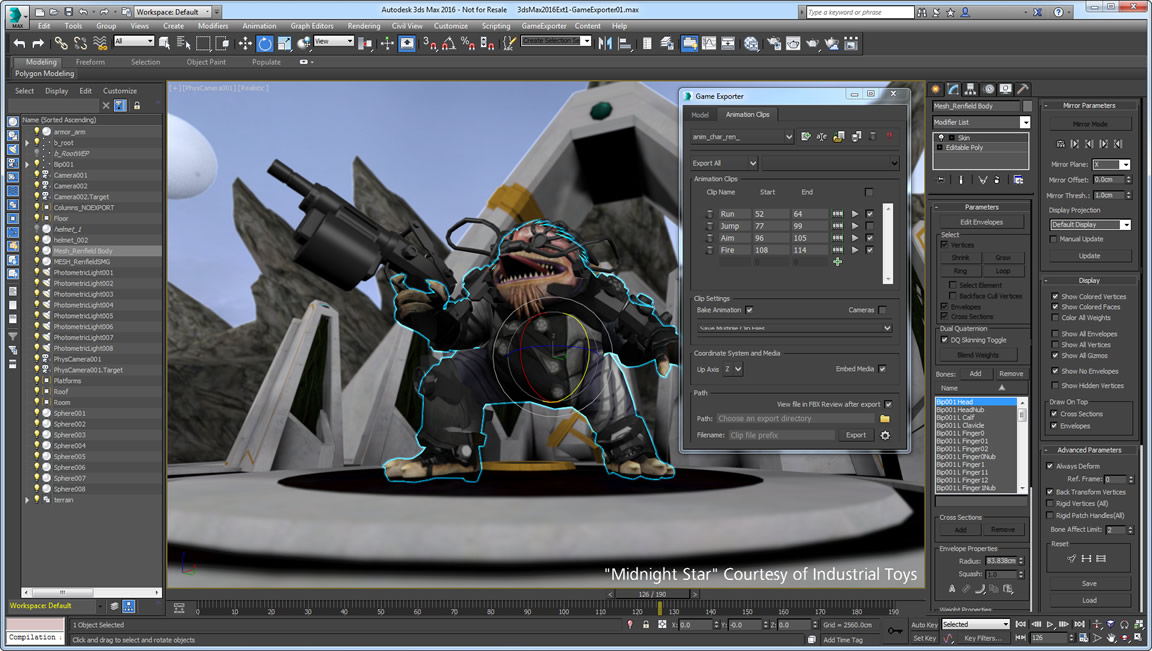
\includegraphics[width=0.9\textwidth]{imagenes/2/3ds-max.jpg}
\caption{Captura de pantalla del entorno de trabajo de 3Ds Max}
\label{fig:3ds-max}
\end{center}
\end{figure}

\subsection{Desarrollo}

Actualmente existen varios entornos de desarrollo integrado, o \acs{IDE} por sus siglas en inglés, destinados a facilitar el desarrollo de videojuegos. En esta sección se presenta los más importantes.

\subsubsection{Unity3D}

Unity es un motor de videojuego multiplataforma creado por Unity Technologies disponible para los principales sistemas operativos, y permite compilar para varias plataformas cómodamente. 

La compañía Unity Technologies fue fundada en 2004 en Dinamarca, la cual desarrolló Unity para su primer juego, \textit{GooBall}, que fue un fracaso. Aún así, los integrantes de la compañía reconocieron el valor del motor de juegos que había hecho y decidieron continuar con su desarrollo hasta lanzar oficialmente Unity un año después, en 2005.  

A día de hoy existen dos versiones; Unity Personal, una versión gratis de Unity para principiantes que no incluye servicio al cliente, capacitación ni servicios adicionales, y Unity Pro, que sí los incluye, costando 125\$ al mes. Además, los desarrolladores de un juego ingrese más de 100,000\$ al año deberán suscribirse a la versión Pro obligatoriamente. En total, más de cinco millones de personas han utilizado Unity en 2017\footnote{\url{https://unity3d.com/public-relations}}.

\begin{figure}[!h]
\begin{center}
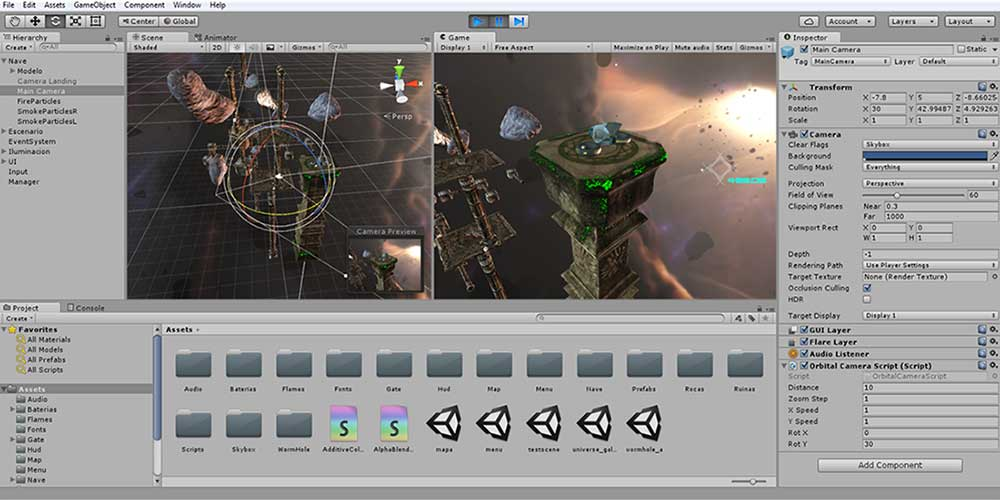
\includegraphics[width=0.9\textwidth]{imagenes/2/unity.jpg}
\caption{Captura de pantalla de un proyecto en Unity}
\label{fig:unity}
\end{center}
\end{figure}


\subsubsection{Unreal Engine}

Unreal Engine es un motor de juego creado por la compañía Epic Games que al estar escrito en C++ presenta un alto grado de portabilidad, por lo que es una de las herramientas más utilizadas por los desarrolladores de juegos.

Este motor fue mostrado inicialmente en el juego de disparos en primera persona \textit{Unreal} en 1998, que incluía detección de colisiones, IA y herramientas para trabajar con juegos en red. El motor se reescribió y cuatro años después se lanzó su segunda versión, que incluía físicas para vehículos y sistemas de partícula, además de soporte para PlayStation 2 y XBox.

Poco a poco, y gracias al éxito de este \acs{IDE}, a lo largo de los años ha ido aumentando sus características y añadiendo soporte para las tarjetas gráficas y videoconsolas que han ido apareciendo.

Desde marzo de 2015 Unreal Engine 4 está disponible públicamente de forma gratuita aunque, si se decide comercializar el juego, la desarrolladora deberá aportar el 5\% de los ingresos que obtenga a Epic\footnote{\url{https://www.unrealengine.com}}.

\begin{figure}[!h]
\begin{center}
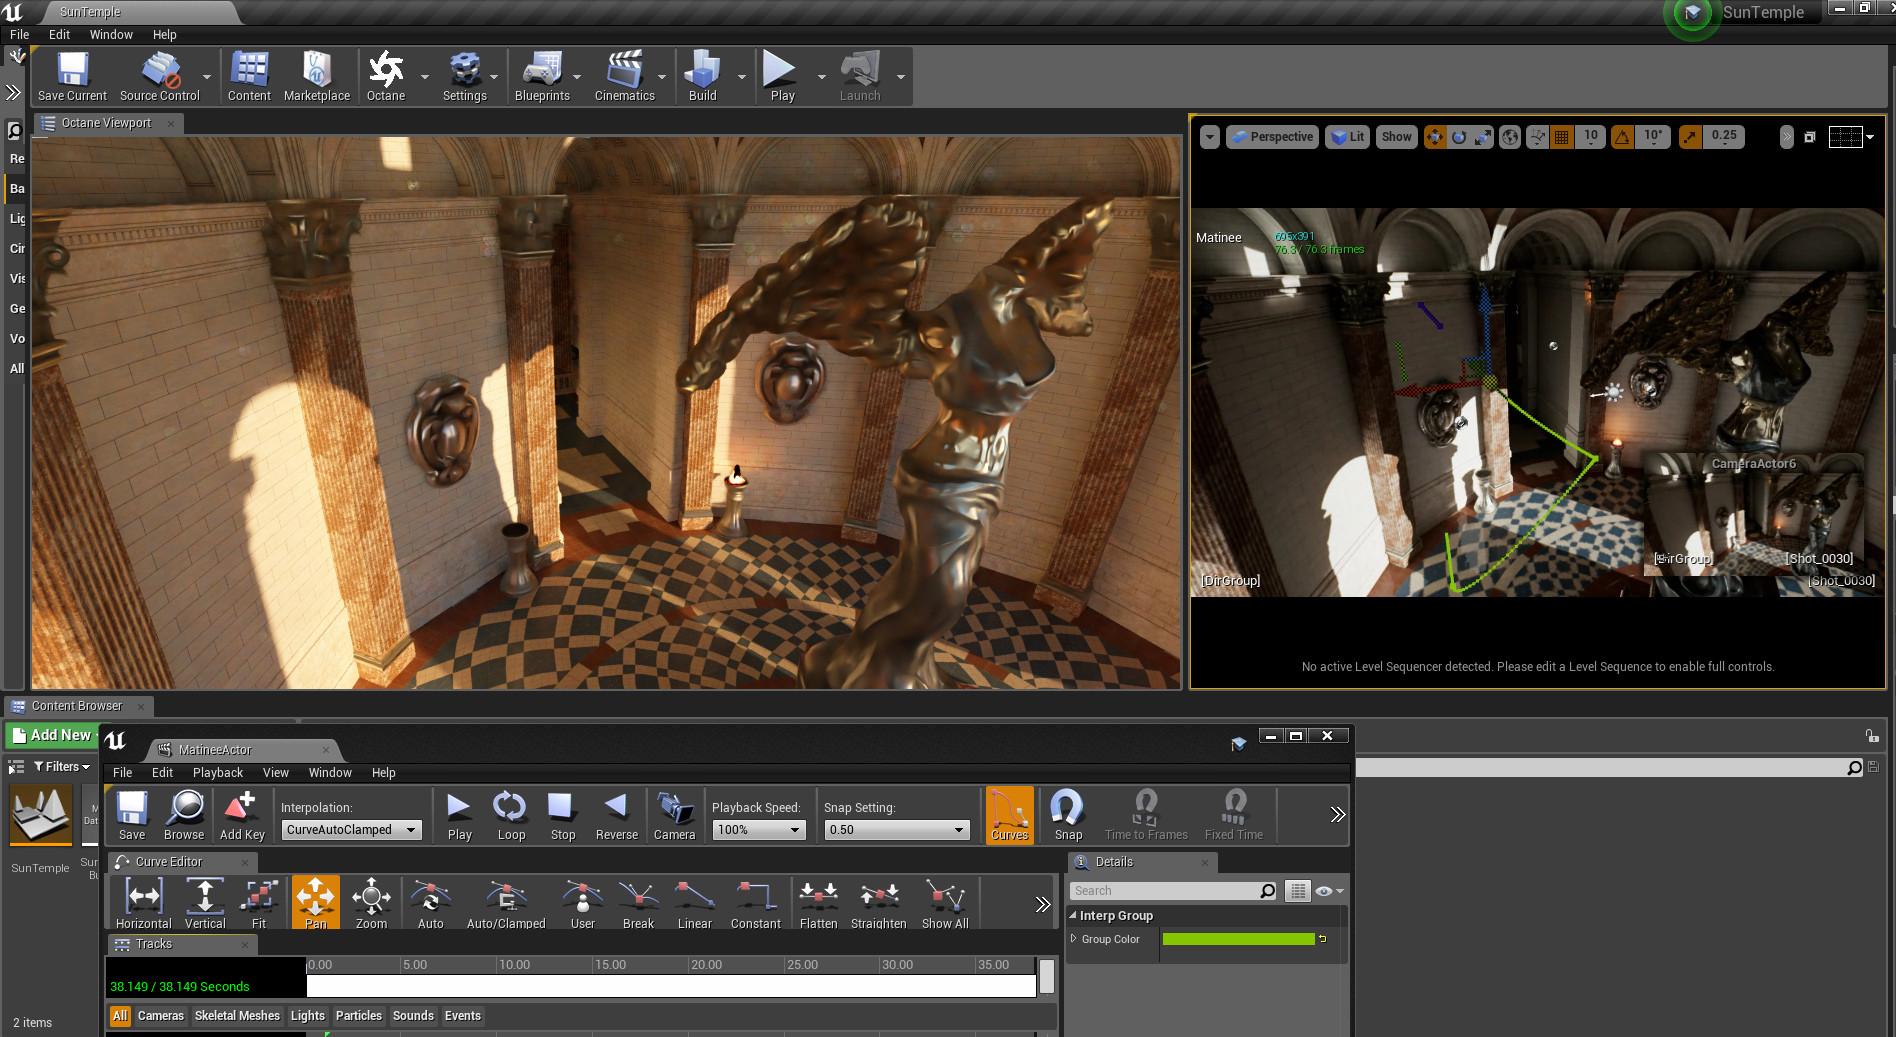
\includegraphics[width=0.9\textwidth]{imagenes/2/unreal-engine-4.jpg}
\caption{Captura de pantalla de un proyecto en Unreal Engine}
\label{fig:unreal}
\end{center}
\end{figure}

\subsubsection{Godot}

Godot es un motor de videojuegos 2D y 3D \textit{open source} publicado bajo la licencia \acs{MIT} desarrollado por su comunidad y disponible para los principales sistemas operativos.

Godot fue desarrollado y utilizado privativamente por la empresa argentina OKAM Studios desde principios del 2001, aunque en febrero de 2014 su código fuente fue liberado y publicado en GitHub\footnote{\url{https://github.com/godotengine/godot}}. Es el principal motor de videojuegos \textit{open source}, y su comunidad ayuda activamente a desarrollarlo. 

Además, actualmente tiene una página en Patreon\footnote{\url{https://www.patreon.com/godotengine}} con más de 1,000 mecenas y obtiene más de 10,000\$ al mes.

\begin{figure}[!h]
\begin{center}
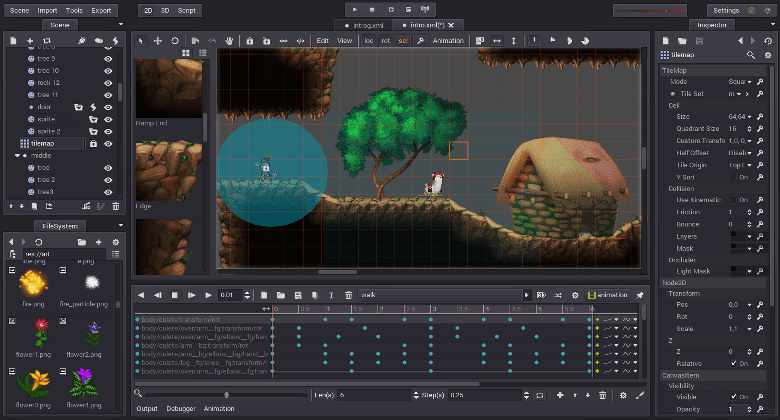
\includegraphics[width=0.9\textwidth]{imagenes/2/godot.jpg}
\caption{Captura de pantalla de un proyecto en Godot}
\label{fig:godot}
\end{center}
\end{figure}

\section{Desarrollo de videojuegos}

El desarrollo de videojuegos es el proceso de creación de un videojuego desde su concepción inicial hasta su versión final. Es una actividad multidisciplinar que involucra profesionales de distintos campos, como programadores, diseñadores gráficos, animadores o compositores de música, entre otras áreas.

A principios de la década de 1960 comenzaron a desarrollarse los primeros videojuegos, pero no estaban disponibles para el público general ya que éste no poseía dispositivos para ejecutarlos dado su elevado precio. No fue hasta la década de 1970 y la llegada de la primera generación de consolas de videojuegos y ordenadores domésticos, como el Apple I, cuando empezaron a desarrollarse videojuegos a nivel comercial. Además, como los ordenadores tenían muy poca potencia y los juegos eran muy simples, un único programador podía hacerse cargo del juego completo en no más de 6 meses \cite{next-gen-97}.

Sin embargo, la creciente potencia de procesamiento de los ordenadores, los estándares de la industria y las expectativas del jugador han hecho que esto deje de ser la norma y solo pase en casos aislados. El precio promedio de la producción de un videojuego lentamente aumentó de 1-4 millones de dólares en 2000 a más de 5 millones en 2005, y luego a más de 20 millones en 2010\footnote{\url{https://en.wikipedia.org/wiki/Video_game_development}}.

Uno de los documentos más importantes, si no el más, a la hora de desarrollar un videojuego es el \textbf{\acl{GDD}}, o por sus siglas en inglés \acs{GDD} a partir de ahora. Este es un documento creado y editado por el equipo de desarrollo  del juego y contiene toda la descripción del videojuego y se utiliza para organizar esfuerzos dentro de un equipo de desarrollo. Este documento no es el guión del juego, sino una síntesis que propone lo que va a ser para que todo el mundo tenga la misma idea en mente \cite{bet-03}. Es equivalente a la \textbf{Biblia} de una serie de televisión. 

Como podemos ver, el desarrollo de un videojuego ha ido adquiriendo un carácter mucho más formal, por lo que que se necesita coordinar a muchos profesionales teniendo en cuenta salarios y tiempos para que el producto final pueda generarse correctamente. En el capítulo \ref{chap:metodologias} se discutirá en mayor profundidad las actuales metodologías de desarrollo que existen y cómo se ha adaptado este proyecto a ellas.

\section{Conclusiones}

A lo largo de este capítulo se han presentado las principales áreas y tecnologías en las que se ha basado este proyecto y que deberán trabajar conjuntamente y hacer sinergia para su correcta completitud.

El papel de la Historia del Arte es principal en este proyecto; tanto su temática como su narrativa están estrechamente a este área, y la estética de cada una de las salas se verá altamente influenciada por la etapa artística que representa.

Por otro lado, el componente inmersivo de la Realidad Virtual es de esencial importancia, y se utilizará junto a la naturaleza motivadora de los videojuegos para hacer que todos los usuarios se sientan totalmente inmersos en el mundo virtual que les ofrece \textit{MineRVa}. Este mundo será modelado completamente a mano, por lo que la  utilización de técnicas y tecnologías de diseño 3D es de vital importancia.